%!TEX root = ../thesis.tex
%*******************************************************************************
%*********************************** Analysis Overview *********
%*******************************************************************************

%\titleformat{\chapter}[display]
%	{\normalfont\LARGE}
%	{\filleft\MakeUppercase{\chaptertitlename}\hspace{0.5cm}\rlap{\resizebox{!}{1.5cm}{\thechapter}~\rule{5cm}{1.5cm}}\hspace{2.0cm}}
%  	{10pt}
%  	{\bf\LARGE\filright}
%\titlespacing*{\chapter}{0pt}{30pt}{20pt}


\chapter{Simplified likelihoods}\label{ch:simplify}

\ifpdf
    \graphicspath{{chapter-simplify/Figs/Raster/}{chapter-simplify/Figs/PDF/}{chapter-simplify/Figs/}}
\else
    \graphicspath{{chapter-simplify/Figs/Vector/}{chapter-simplify/Figs/}}
\fi

In the previous chapter, the concept of preserving an analysis for the purpose of reinterpretations was introduced and a truth-level version of the signal pipeline was discussed. In large-scale reinterpretations involving a large number of \gls{susy} models to be tested against, not only the signal pipeline, but also the statistical inference requires significant computational effort. 
This chapter therefore introduces the concept of \textit{simplified likelihoods}, a method approximating the statistical model of an analysis using the \lib{HistFactory} template in order to achieve more efficient log-likelihood fits and, ultimately, hypothesis tests.

\section{Motivation}\label{sec:simplified_likelihood_motivation}

\begin{figure}
	\centering
	\begin{subfigure}[b]{0.5\textwidth}
		\centering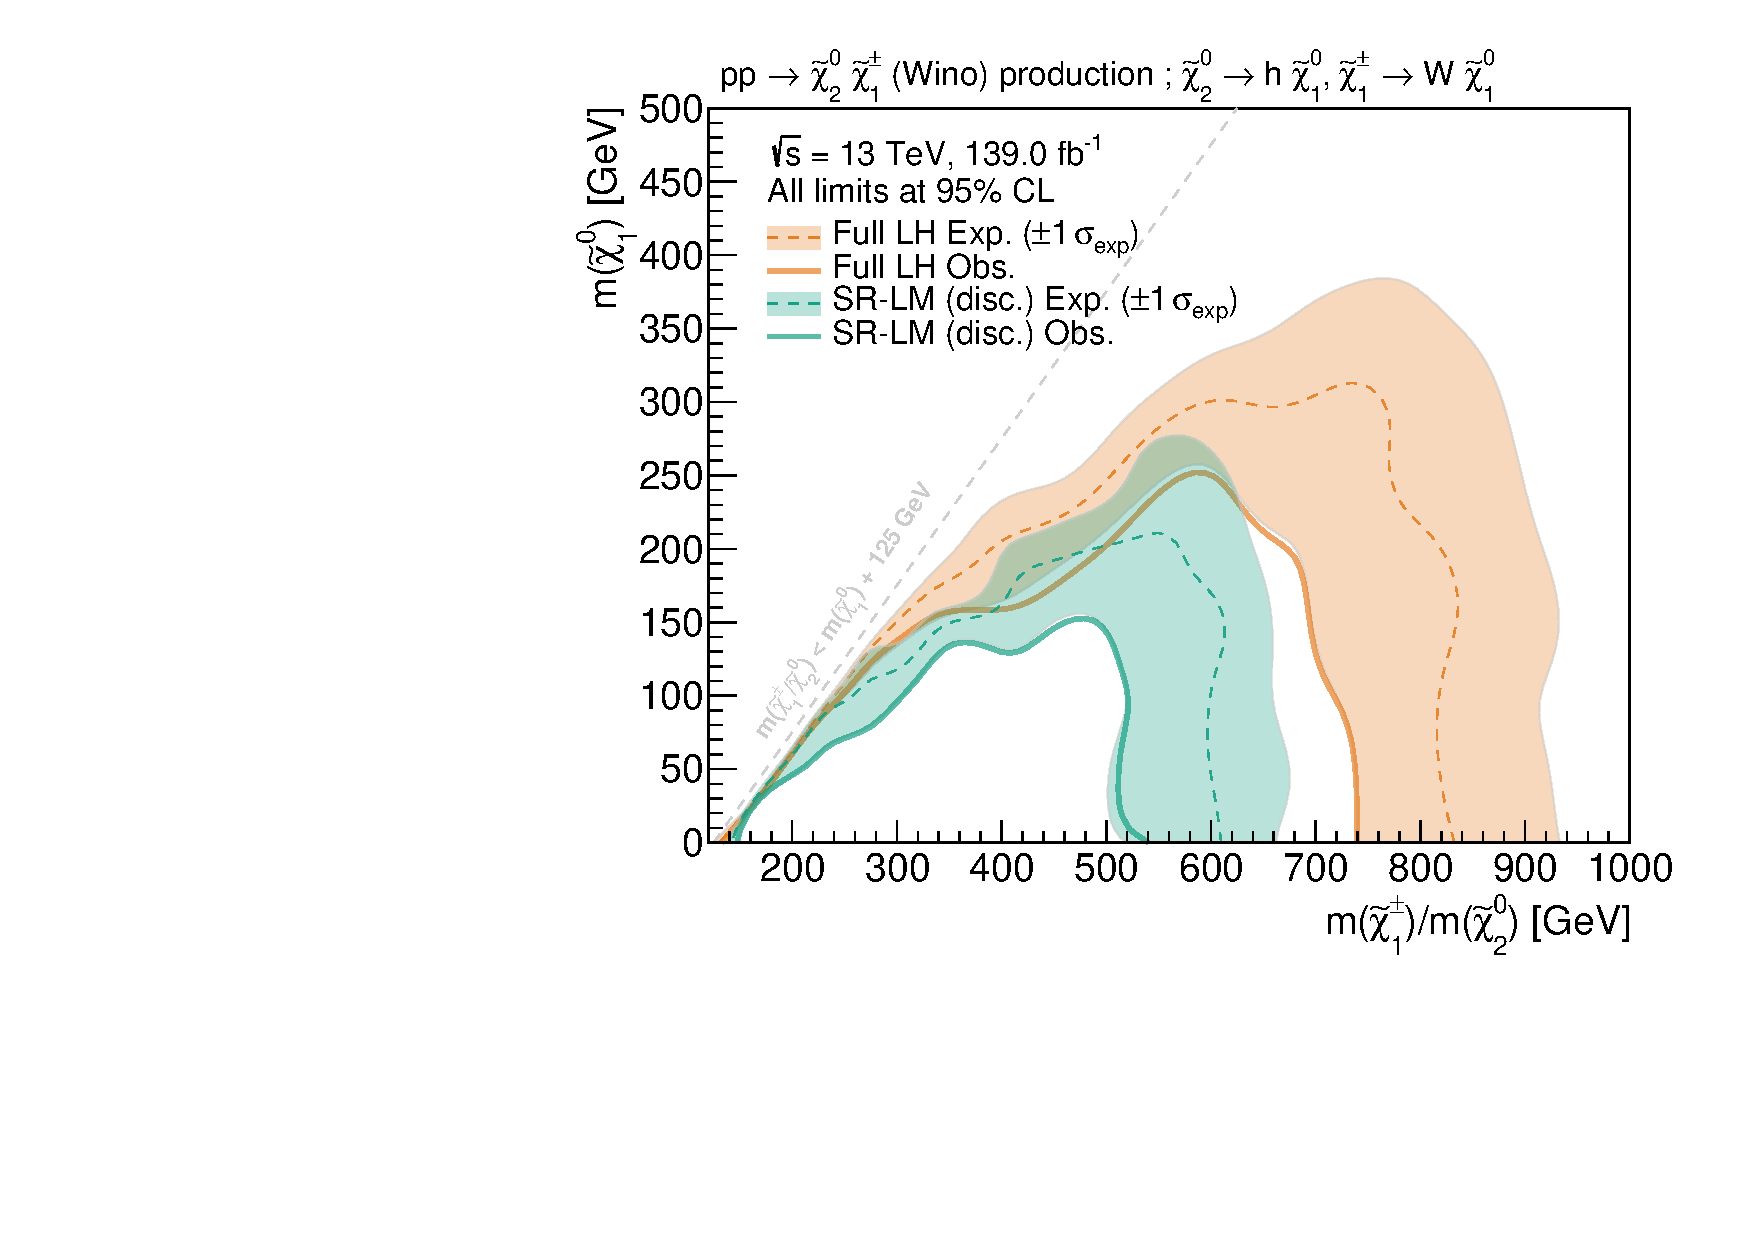
\includegraphics[width=\textwidth]{exclusion_1Lbb_SRLM_noLabel_v2}
		\caption{Discovery SR-LM\label{fig:single_bin_SRLM}}
	\end{subfigure}\hfill
	\begin{subfigure}[b]{0.5\textwidth}
		\centering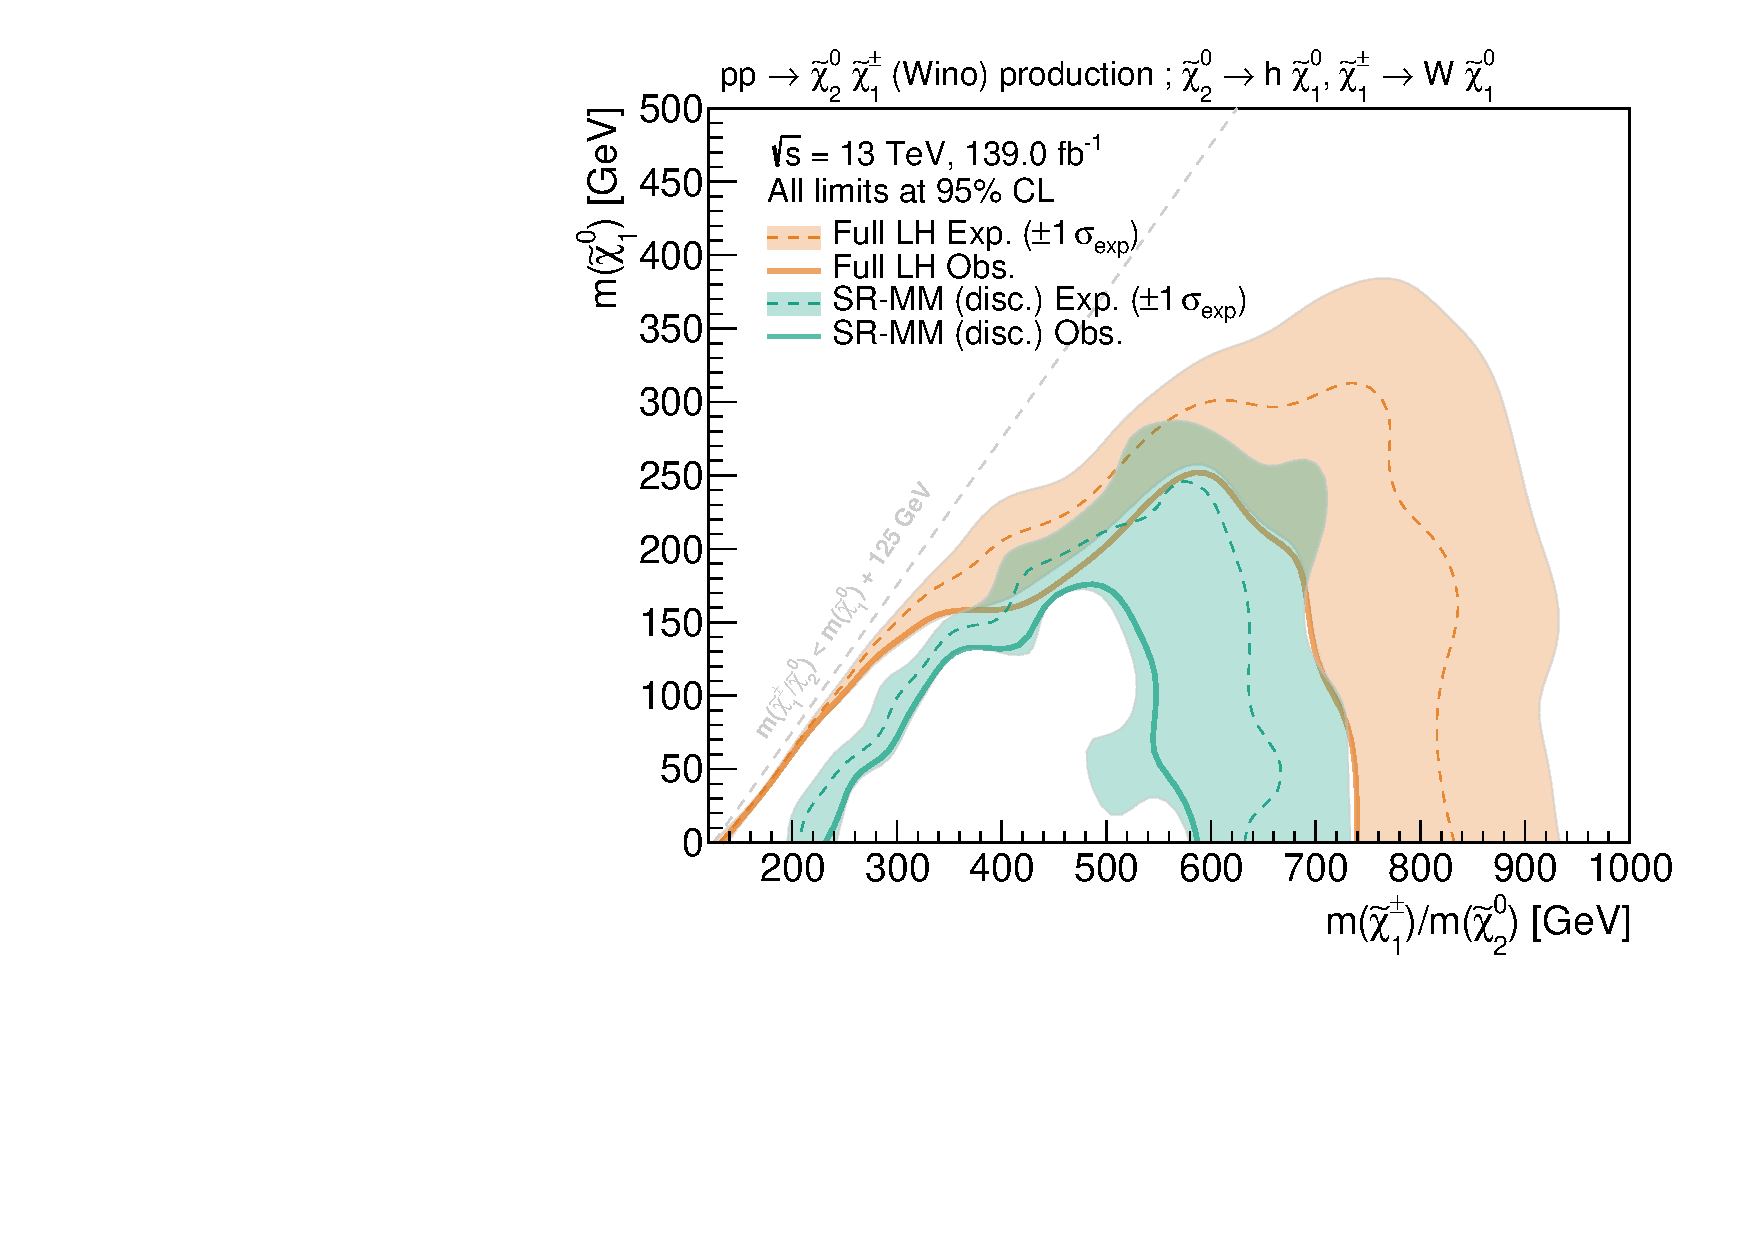
\includegraphics[width=\textwidth]{exclusion_1Lbb_SRMM_noLabel_v2}
		\caption{Discovery SR-MM\label{fig:single_bin_SRMM}}
	\end{subfigure}\hfill
	\par\medskip
	\begin{subfigure}[b]{0.5\textwidth}
		\centering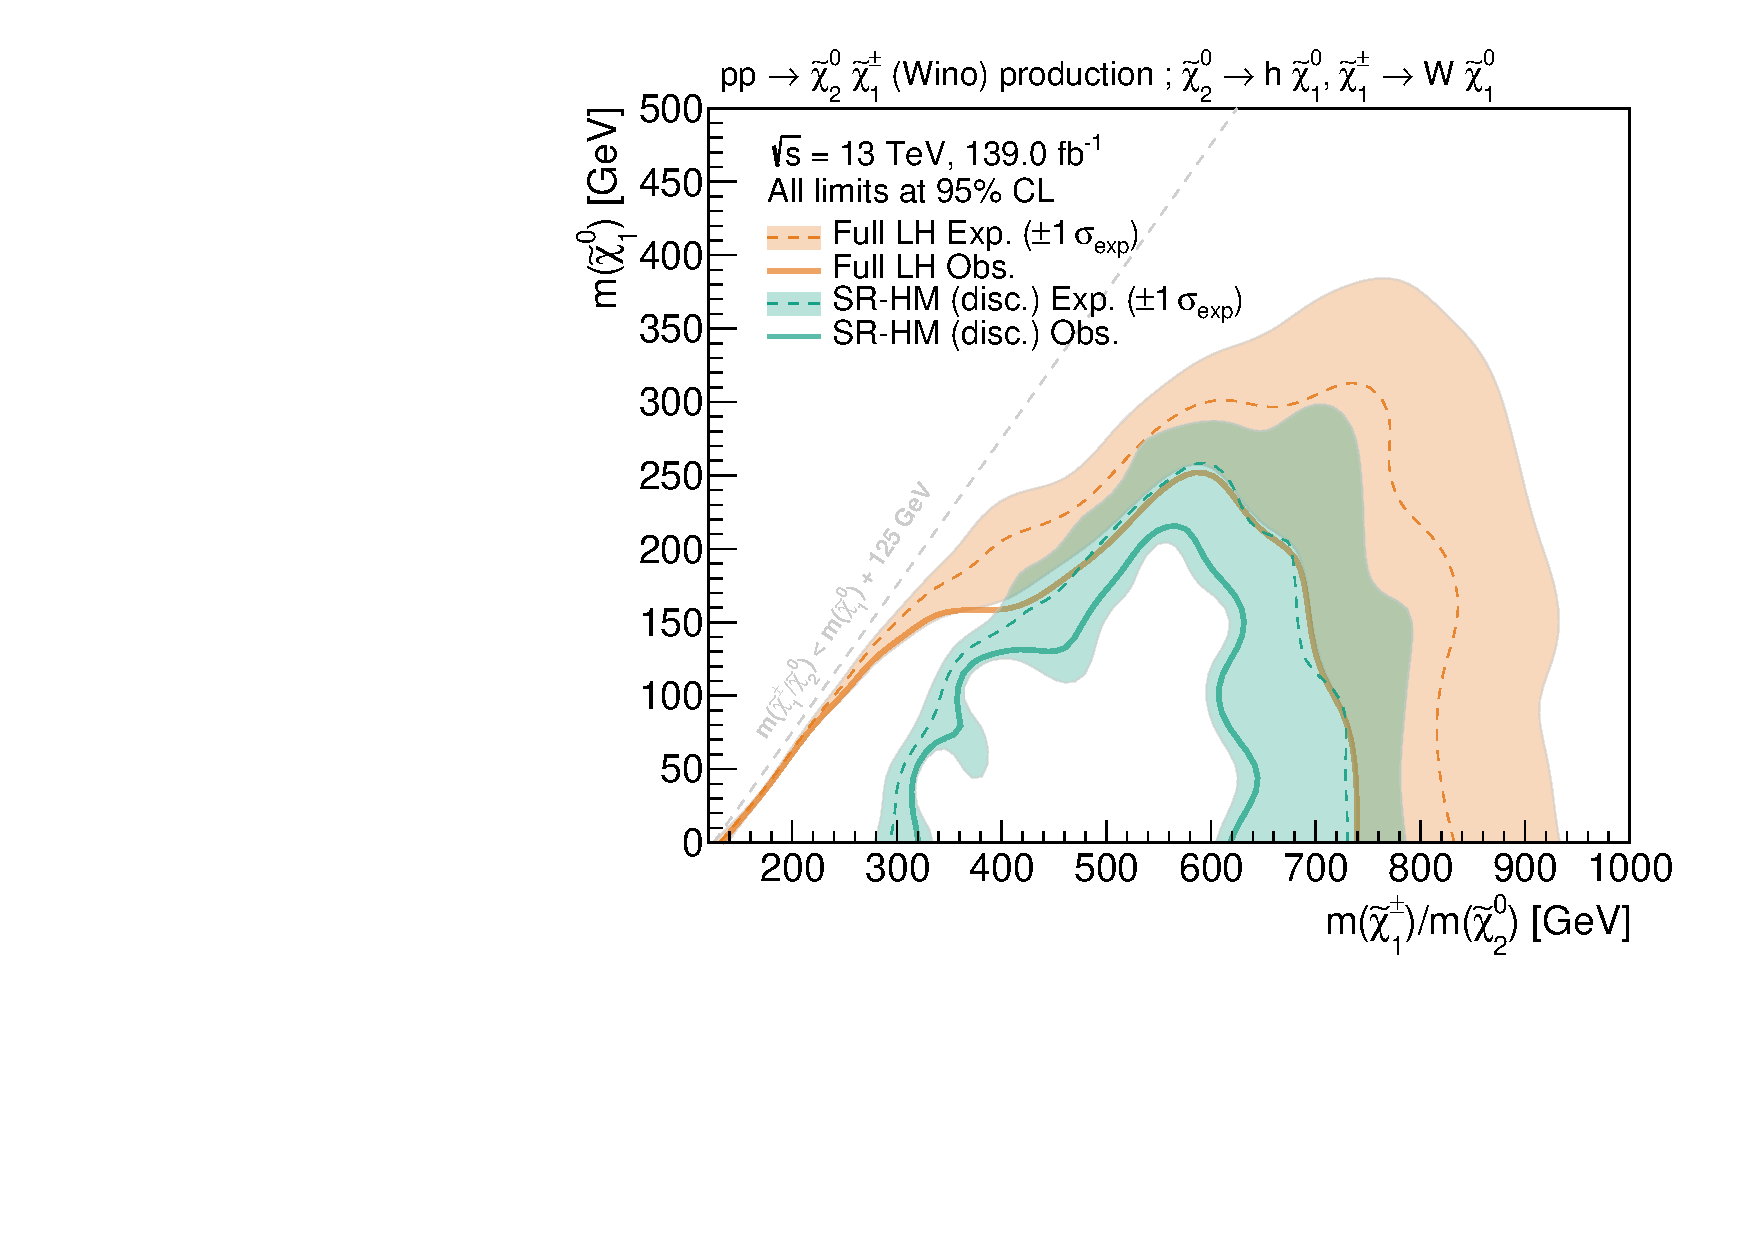
\includegraphics[width=\textwidth]{exclusion_1Lbb_SRHM_noLabel_v2}
		\caption{Discovery SR-HM\label{fig:single_bin_SRHM}}
	\end{subfigure}%
	\caption{Comparison of exclusion limits obtained using a likelihood built from all nine exclusion signal regions (orange), and the discovery signal regions (green). As discussed in~\cref{sec:signal_region_definitions}, the discovery signal regions are simple \textit{cut-and-count} regions making minimal model assumptions. As they are not mutually exclusive, they cannot be statistically combined, thus resulting in three separate exclusion contours. All statistical and systematic uncertainties on the background and the signal event rates are included in all regions.}\label{fig:single_bin}
\end{figure}

Reinterpretations of ATLAS searches for \gls{susy} in more complete and realistic \gls{susy} scenarios (as opposed to simplified models) typically involve high-dimensional parameter spaces that are computationally extremely challenging to sample and compare to ATLAS data in an exhaustive manner.
Large-scale reinterpretations of this type have already been performed in ATLAS after the Run~1 data-taking period in both the full 19-dimensional \gls{pmssm}~\cite{pMSSM-scan-run1:2015baa} as well as a 5-dimensional representation of the \gls{pmssm} focussing on the electroweak sector~\cite{Aaboud:2016wna}.
Due to the complexity of the statistical models of today's ATLAS searches for \gls{susy}, originating from the large number\footnote{As an example, the full likelihood of the \onelepton search using the exclusion signal regions has 8 channels with a total of 14 bins. Each channel gets event rates for 9 samples that depend on a total of 115 modifiers.} of channels and the sizeable set of nuisance parameters usually considered, the wall time needed for the statistical inference is usually not negligible.
In a typical large-scale reinterpretation involving \mbox{$\mathcal{O}(10^5$--$10^6)$} sampled models, an optimistic estimation of the wall time needed for the statistical inference per model of \mbox{$\mathcal{O}(\SI{10}{\second}$--$\SI{e2}{\second})$} is too computationally expensive, especially when more than just a single ATLAS search is included.
It is thus crucial to reduce the number of models that need to be evaluated using the searches' full statistical model.

One approach of alleviating this computational problem is to approximate the \gls{susy} searches through their model-independent upper limits, often published in conjunction with the model-dependent exclusion limits.
As discussed in \cref{sec:signal_region_definitions}, the model-independent upper limits are derived using single-bin signal regions that do not rely on shape-fits but simply count the numbers of events after a set of selection cuts (so-called \textit{cut-and-count} regions), thereby making minimal model assumptions.
In the case of searches using dedicated multi-bin signal regions that are statistically combined to derive exclusion limits on model parameters, this approach---while computationally very efficient---naturally underestimates the true exclusion power of the respective search since model-dependent signal shapes are not exploited.

\Cref{fig:single_bin} illustrates this approach in the context of the \onelepton search. The exclusion limits obtained with the exclusion signal regions implementing a two-dimensional shape-fit are compared to the exclusion contours obtained using the discovery signal regions, defined in~\cref{tab:SignalRegionDef}.
As the discovery signal regions are not mutually exclusive, they cannot be statistically combined and thus three separate observed and expected contours need to be drawn. It can be observed that even a best-expected combination of the three discovery signal regions does not reach the sensitivity achieved using the two-dimensional shape-fit setup, resulting from the statistical combination of the nine exclusion signal regions.
In the past, such approaches were used nonetheless in large-scale scans of the \gls{pmssm} using ATLAS data from Run~1~\cite{pMSSM-scan-run1:2015baa,Aaboud:2016wna}, yielding conservatives results and thus leaving substantial room for improvement.

Hence the motivation to introduce a method for approximating ATLAS searches for \gls{susy} without disregarding their elaborate use of multi-bin signal regions exploiting the varying shapes of signal and \gls{sm} background distributions. The method introduced hereafter targets ATLAS searches for \gls{susy} using likelihoods built according to the \lib{HistFactory} template.

\section{Building simplified likelihoods}\label{sec:building_simplified_likelihoods}

In order to retain the full statistical combination of multiple signal region bins implemented in many SUSY searches, while still being able to achieve a sufficiently fast approximation, the statistical treatment of the background model including its uncertainties needs to be simplified.
In the procedure presented in the following, this is achieved by first performing a background-only fit to data using the full likelihood in order to determine the best-fit values of all model parameters $\boldsymbol{\phi}$.
The post-fit total background estimate as well as the total uncertainty on the estimate in every bin are subsequently computed from the best-fit values, and used to construct a simplified likelihood.

As the full likelihood in \texttt{JSON} format defines the full statistical model used for the statistical inference, the above background-only fit can be performed using \texttt{pyhf} and the preserved likelihood of the analysis.
With the full likelihoods starting to become available on \lib{HEPData} (see \eg \reference\cite{fullLH_1Lbb}) this procedure can rely on public information only and is therefore widely accessible to the \gls{hep} community.
The simplified likelihoods introduced herein follow the same \texttt{JSON} specification used for the full likelihoods, described in \reference\cite{ATL-PHYS-PUB-2019-029}.
The following description highlights the specification details relevant to the simplified likelihood. 

\subsubsection{Background model}

In the simplified likelihood, the background model is approximated with a single background sample, called \texttt{total\_bkg} in \cref{lst:bkg_sample} and representing the total \gls{sm} background estimate in the different analysis channels.
The pre-fit sample rate of the total background sample is set to the total post-fit background estimate obtained in the background-only fit using the full likelihood (in \cref{lst:bkg_sample} set to be $10.0$).
Furthermore, the complete set of nuisance parameters in the original full likelihood is reduced to a single constrained parameter $\alpha$ with up and down variations corresponding to the post-fit uncertainties on the total \gls{sm} background estimates in each bin.
In \cref{lst:bkg_sample}, the single nuisance parameter is called \texttt{total\_error} and is implemented as a rate modifier (introduced in \cref{sec:likelihood_function}).
It is constrained by a Gaussian of the form $\mathrm{Gaus}(a = 0 \vert \alpha , \sigma = 1)$ and is correlated over all bins in each channel. The $1\sigma$ up and down evaluations of the rate modification, necessary for the interpolations during the log-likelihood fit to data, are given by the post-fit uncertainties on the total background estimate.

Although the final uncertainty is thus constrained by a simple Gaussian, the full treatment of the uncertainties including all correlations using the full likelihood in order to derive the in pre-fit values in the simplified likelihood, ensures that non-Gaussian effects are included to some extent.

\begin{minipage}{\linewidth}
\begin{lstlisting}[language=json,firstnumber=1,caption={Example of a total background sample with sample rate and total uncertainty as derived from a previous fit in the \glspl{sr} and \glspl{cr}. The `\textit{histosys}' type modifier in \lib{HistFactory} implements a shape uncertainty correlated over all bins.},captionpos=b, label=lst:bkg_sample]
{
	"name": "total_bkg",
	"data": [10.0],
	"modifiers": [{
		"data": {"hi_data": [12.0], "lo_data": [8.0]}, 
		"name": "total_error", "type": "histosys"
	}]
}
\end{lstlisting}
\end{minipage}

\subsubsection{Analysis channels}

Each channel in the full likelihood with the original number of bins is also entering the simplified likelihood\footnote{Being able to reproduce the full statistical combination of all analysis regions is one of the main motivations for the introduction of the simplified likelihood.}. Each contains the total background sample as specified above.
Apart from the total background sample, one additional sample is needed: the signal sample, an example of which is shown in \cref{lst:sig_sample}.
It introduces the unconstrained signal strength parameter $\mu$ as second and final parameter of the likelihood.
For simplicity, the example shown in \cref{lst:sig_sample} does not introduce any additional uncertainties on the signal rates, thereby assuming them to be negligible. Depending on the \gls{bsm} scenario, signal uncertainties can, however, be introduced through additional event rate modifiers.

\begin{minipage}{\linewidth}
\begin{lstlisting}[language=json,firstnumber=1,caption={Example of a signal sample with sample rate and unconstrained normalisation parameter that will be used as \gls{poi}.},captionpos=b, label=lst:sig_sample]
{
	"name": "signal",
	"data": [7.0],
	"modifiers": [{"data": null, "name": "mu", "type": "normfactor"}]
}
\end{lstlisting}
\end{minipage}

\subsubsection{Observations and measurements}

According to the \texttt{JSON} specification defined in \reference\cite{ATL-PHYS-PUB-2019-029}, the data observed by the analysis in each channel (and each bin) is introduced by means of an \textit{observation}. In the case of the simplified likelihood, this is taken directly from the full likelihood and, by construction, does not need to be modified in any form. An example of an observation including several channels and bins is shown in~\cref{lst:observation}.

\begin{minipage}{\linewidth}
\begin{lstlisting}[language=json,firstnumber=1,caption={Example of an observation in the simplified likelihood. It can be taken directly from the corresponding full likelihood. This example implements three channels, two with one bin, and one with three bins. The number of events observed in data are given for each channel and bin.},captionpos=b, label=lst:observation]
{
	"observations": {
		{"name": "channel_A" : "data": [25.0]},
		{"name": "channel_B" : "data": [20.0]},
		{"name": "channel_C" : "data": [11.0, 13.0, 21.0]}
	}	
}
\end{lstlisting}
\end{minipage}

The only part of the \texttt{JSON} specification left to be defined is the \textit{measurement}, specifying the name of the parameter of interest as well as parameter set configurations not already covered in the channel definitions. For the simplified likelihood, it is straightforward to write down, as the \gls{poi} is the signal strength parameter and no additional parameters need further configuration. An example measurement is shown in \cref{lst:measurement}.

\begin{minipage}{\linewidth}
\begin{lstlisting}[language=json,firstnumber=1,caption={Example of a measurement in the simplified likelihood. The signal strength is the parameter of interest, no additional parameters need further configuration.},captionpos=b, label=lst:measurement]
{
	"measurements": {
		"name": "myMeasurement",
		"config": { "poi": "mu", "parameters": []}
	}	
}
\end{lstlisting}
\end{minipage}

Put together, the above pieces result in a simplified likelihood for a given signal model, using a background model obtained from an initial background-only using the full likelihood, thus considering the full treatment of the systematic uncertainties.
The simplified likelihood approach thus assumes the total background estimate to be fixed at the post-fit values obtained from the initial full likelihood fit, and only allowed to vary in a correlated way within the total uncertainty.

All simplified likelihoods used in the following have been produced using \pylib{simplify}~\cite{simplify}, a \texttt{python} tool written by the author.
The background model of the simplified likelihood of the \onelepton search in \texttt{JSON} format is available at \reference\cite{simplified_lh_SUSY-2019-08}.
By the means of \texttt{JSON} patches~\cite{json_patch}, any signal model, for which the nominal expected event rates in the analysis regions are known, can then be evaluated using this simplified likelihood.


\section{Computational performance}\label{sec:cpu_performance}

One of the main figures of merit of an analysis approximation naturally is the reduction in computational wall time compared to the full analysis. \Cref{fig:benchmark_1Lbb} shows a benchmark for different likelihood configurations in the context of the \onelepton search.
The wall times of hypothesis tests using the full analysis likelihood are compared with those using the simplified likelihood constructed following the previously introduced prescription.
In addition, the wall time of the single-bin likelihood using the discovery \glspl{sr} already used in \cref{fig:single_bin}, is shown.
For each likelihood, different computational backends are used for the tensor algebra operations in \texttt{pyhf}. All benchmarks have been performed on an Intel i7-4790 CPU with a nominal clock speed of $\SI{3.60}{\GHz}$, 4 cores and 8 threads.
The CPU was not isolated, but under minimal load.
The original 125 signal points of the \onelepton search were used in each configuration.

\begin{figure}
	\centering    
	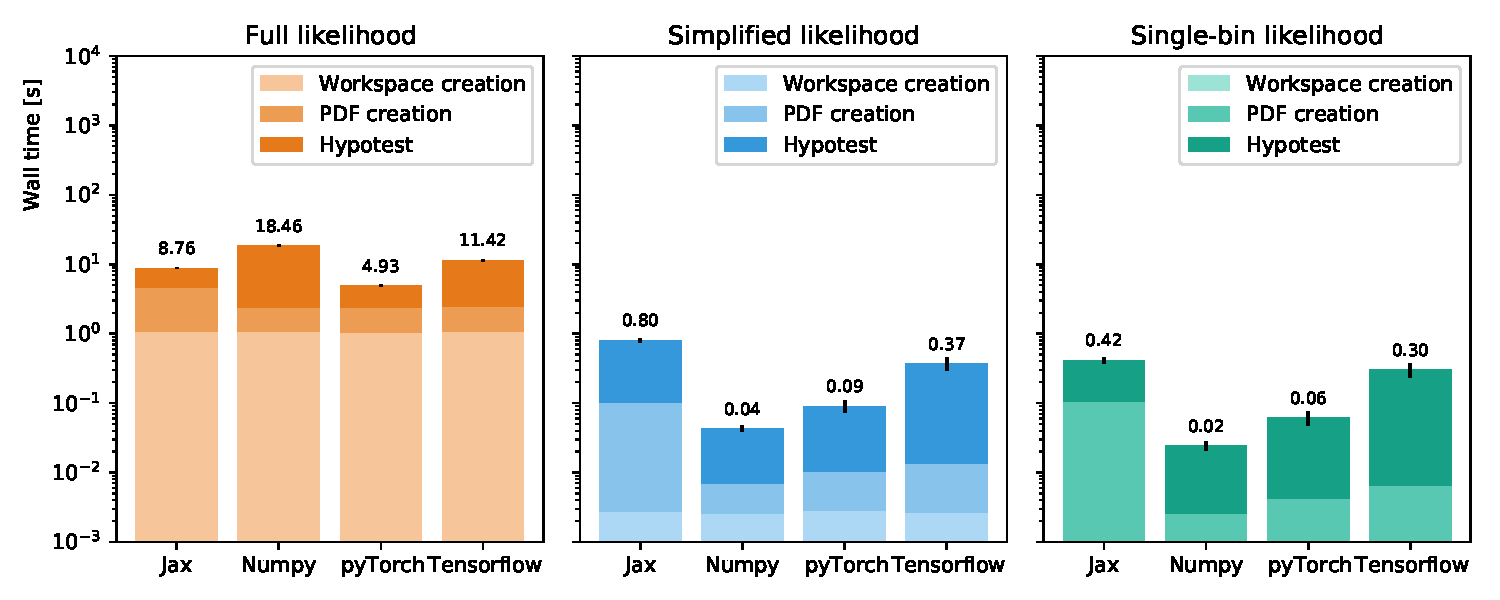
\includegraphics[width=0.95\textwidth]{benchmark_1Lbb}
	\caption{Benchmarks of the wall times necessary for hypothesis testing using different likelihoods and \texttt{pyhf} backends in the context of the \onelepton search. Benchmark details are given in the text. The full likelihood (left) includes the full statistical implementation of the original analysis, the simplified likelihood (center) represents the simplified likelihood approach presented in this document, and the single-bin likelihood (right) represents the single-bin approximation using the discovery signal regions. The uncertainties represent the standard deviation of the benchmark test sample. The `\textit{workspace creation}` refers to I/O operations reading in the \texttt{JSON} file containing the likelihood. The `\textit{pdf creation}' step refers to the creation of the statistical model in a \texttt{pyhf}-internal structure, depending already on the computational backend. `\textit{Hypotest}' refers to the wall time of a single exclusion hypothesis test computing a CL$_s$ value. Error bars correspond to the standard deviation of the benchmark sample.}\label{fig:benchmark}
	\label{fig:benchmark_1Lbb}
\end{figure}

\begin{table}
	\begin{center}
	\small
			\begin{tabular} {l r r r}
				\toprule
				Analysis & Full likelihood [s] & Simplified likelihood [s] & Improvement \\
				\midrule
				ATLAS compressed search~\cite{SUSY-2018-16} & $16.49\pm 3.16$ & $0.073 \pm 0.012$ & 236$\times$ \\
				ATLAS $3\ell$ search & $40.41 \pm 15.7$ & $0.082 \pm 0.021$ & 495$\times$\\
				ATLAS $2\ell$ search~\cite{SUSY-2018-32} & $5.93 \pm 0.16$ & $0.079 \pm 0.0082$ & 75$\times$\\
				ATLAS $1\ell$ search~\cite{SUSY-2019-08} & $4.93 \pm 0.11$ & $0.040 \pm 0.0057$ & 123$\times$ \\
				ATLAS direct stau search~\cite{SUSY-2018-04} & $1.91 \pm 0.090$ & $0.039 \pm 0.0055$ & 49$\times$\\
				ATLAS sbottom search~\cite{SUSY-2018-31} & $1.36 \pm 0.067$ & $0.038 \pm 0.0046$ & 36$\times$ \\
				ATLAS stop search & $2.27 \pm 0.062$ & $0.044 \pm 0.011$ & 51$\times$\\
				\bottomrule
			\end{tabular}
		\caption{Benchmarks of the wall times needed for computing the CL$_s$ value for a single signal model using the full and the simplified likelihoods. The signal models used for the benchmarks include all signal models originally considered in the respective searches. The uncertainty corresponds to the standard deviation of the wall times of the benchmark sample. The performance gain is stated as ratio between the wall times. The \pylib{PyTorch} (\pylib{NumPy}) backend of \texttt{pyhf} is used for the full (simplified) likelihood, in conjunction with the \pylib{SciPy} optimiser. Searches without reference quoted are not yet public.}
		\label{tab:simplified_performance}
	\end{center}
\end{table}

The use of automatic differentiation of the full log-likelihood gradient, enabled by some of the tensor algebra backends to \texttt{pyhf}, offers an efficient minimisation of the negative log-likelihood, resulting in fast hypothesis tests of $\mathcal{O}(\SI{5}{\second})$ for the full likelihood.
In large-scale reinterpretations, this is however still too computationally expensive.
The simplified likelihood, on the other hand, yields minimum wall times for hypothesis tests of the order of $\SI{0.04}{\second}$ per signal model.
Compared to the naive single-bin approach using the discovery signal regions (the \textit{single-bin likelihood}), the simplified likelihood thus offers hypothesis tests with a similar wall time\footnote{In fact, the simplified likelihood is actually even faster than the single-bin approach, as the latter needs to be executed separately for each discovery \gls{sr} and thus the numbers quoted need to be multiplied by the number of discovery \glspl{sr} used in the analysis (three in the case of the \onelepton search).}, but a significantly better approximation of the true analysis exclusion power.

Interestingly, the wall time of the simplified likelihood does not benefit from the usage of features like automatic differentiation, offered by backends like \pylib{PyTorch}.
This is due to the extreme simplicity of the simplified likelihood function, causing the computational benefits from features like automatic differentiation to not outweigh the sizeable overhead associated to the startup and execution times of libraries like \pylib{PyTorch}.

In addition to the \onelepton search, the simplified likelihood approach is validated a set of additional ATLAS searches for \gls{susy}. \Cref{tab:simplified_performance} summarises the mean wall times of all ATLAS searches investigated. In all cases, \pylib{PyTorch} offers the fastest backend for the full likelihood while \pylib{NumPy} shows best performance for the simplified likelihood. The performance improvement of roughly two orders of magnitude, observed in the \onelepton search, is confirmed in the other ATLAS \gls{susy} searches investigated. The wall time of the simplified likelihoods appears to be bound from below at $\mathcal{O}(\SI{e-2}{\second})$, limiting the performance gain for some of the faster analyses whose full likelihoods are already relatively simple to begin with.


\section{Physics performance}\label{sec:physics_performance}

\begin{figure}
\floatbox[{\capbeside\thisfloatsetup{capbesideposition={right,center},capbesidewidth=0.30\textwidth}}]{figure}[\FBwidth]
{\caption{Comparison of the simplified likelihood (blue) and full likelihood (orange) exclusion contours for the \onelepton search. The uncertainty band includes all \gls{mc} statistical and systematic uncertainties in the case of the full likelihood, and only the simplified uncertainties in the case of the simplified likelihood.}\label{fig:results_simplify_1Lbb}}
{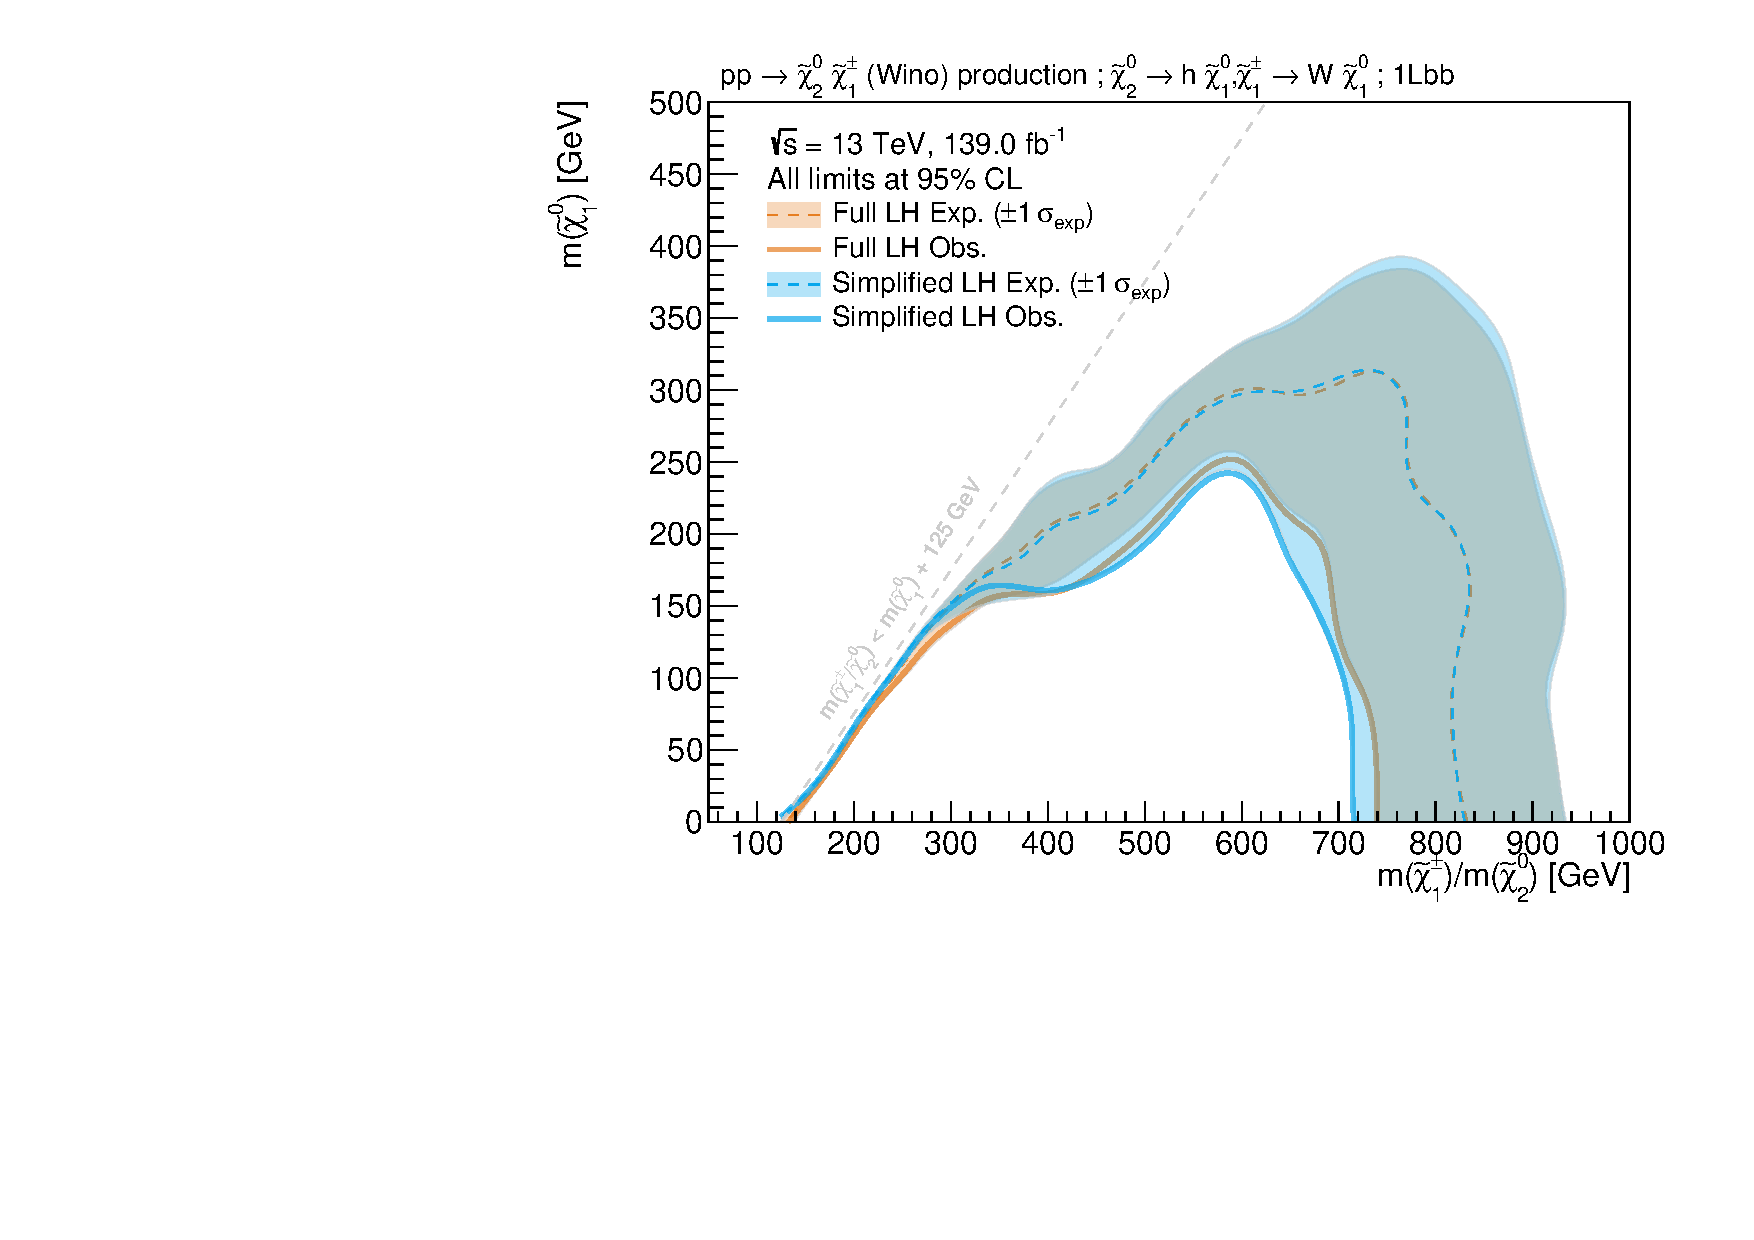
\includegraphics[width=0.65\textwidth]{exclusion_1Lbb_noLabel}}
\end{figure}

A comparison of the exclusion contours obtained with the full and simplified likelihoods in the context of the \onelepton search is shown in~\cref{fig:results_simplify_1Lbb}. The results obtained using the simplified likelihood are shown in blue, while the results obtained using the full likelihood are given in orange. Both the observed (without the usual theoretical up and down variations on the signal cross section) and expected exclusion limits including the uncertainty band are shown. In the case of the full likelihood, the complete set of \gls{mc} statistical and systematic uncertainties introduced in \cref{ch:uncertainties} are taken into account. As discussed in \cref{sec:building_simplified_likelihoods}, the uncertainty band on the simplified likelihood contour results from the single nuisance parameter built through reduction of the original nuisance parameters.

The observed and expected CL$_s$ values obtained using both likelihoods are shown in~\cref{fig:scatter_cls}. As expected from the exclusion contour, both the simplified and the full likelihood agree reasonably well across the majority of the CL$_s$ range. For signal models well within exclusion ($\mathrm{CL}_s \ll 0.05$) based on the full likelihood, the simplified likelihood of the \onelepton search tends to result in slightly lower CL$_s$ values than the full likelihood, yielding a slightly too optimistic sensitivity estimate. In the range relevant to the exclusion contour at 95\% CL (CL$_s\approx0.05$), the results from the simplified likelihood agree however well with those from the full likelihood.

In addition to the \onelepton search, the simplified likelihood approach has been tested on the ATLAS \gls{susy} searches listed in \cref{tab:simplified_performance}. An overview of the results can be seen in~\cref{fig:results_analyses}, comparing the exclusion contours obtained with the simplified likelihood against the full analysis results. In some analyses, \eg, the ATLAS sbottom  and ATLAS $3\ell$ searches, the simplified likelihoods show excellent agreements. In other analyses, like \eg, the ATLAS direct stau search, the agreement is less good but overall still acceptable.
In summary, this demonstrates that the method can, in many cases, offer a fast and reliable approximation of ATLAS searches for \gls{susy} using the \text{HistFactory} template.

\begin{figure}
	\centering
	\begin{subfigure}[b]{0.5\textwidth}
		\centering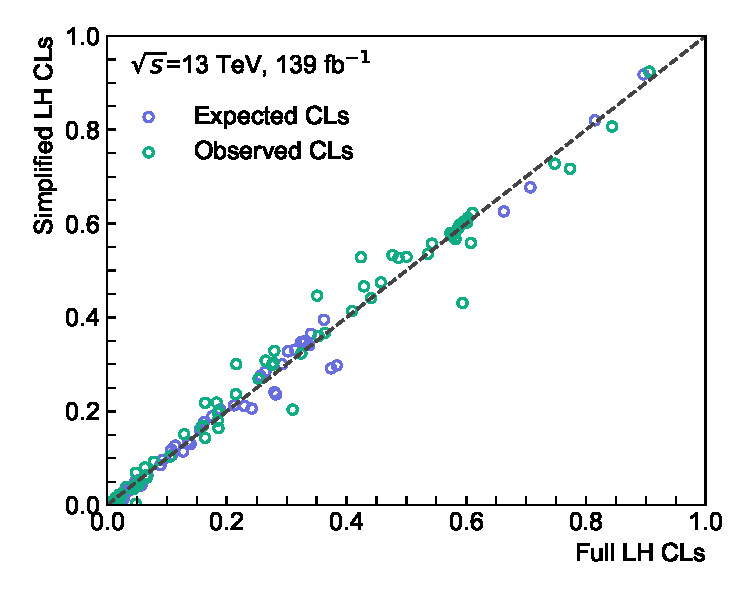
\includegraphics[width=\textwidth]{cls_scatter_1Lbb_lin}
		\caption{Linear scale}
	\end{subfigure}\hfill
	\begin{subfigure}[b]{0.5\textwidth}
		\centering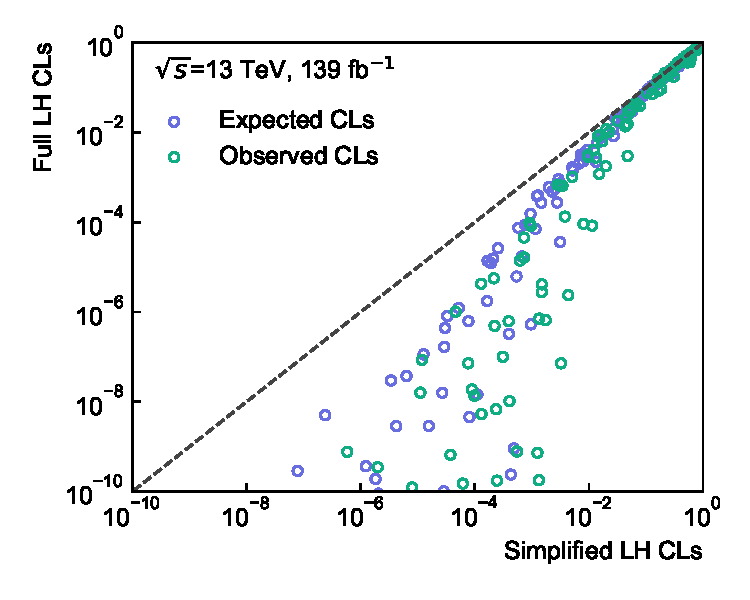
\includegraphics[width=\textwidth]{cls_scatter_1Lbb_log}
		\caption{Logarithmic scale}
	\end{subfigure}
	\caption{Scatter plots comparing the observed and expected CL$_s$ values obtained using the simplified and the full likelihoods for the same set of signal models considered in the \onelepton search. Both linear and logarithmic scale representations are shown to give an overview of the full range of CL$_s$ values.}\label{fig:scatter_cls}
\end{figure}



\begin{figure}
	\centering
	\begin{subfigure}[b]{0.5\textwidth}
		\centering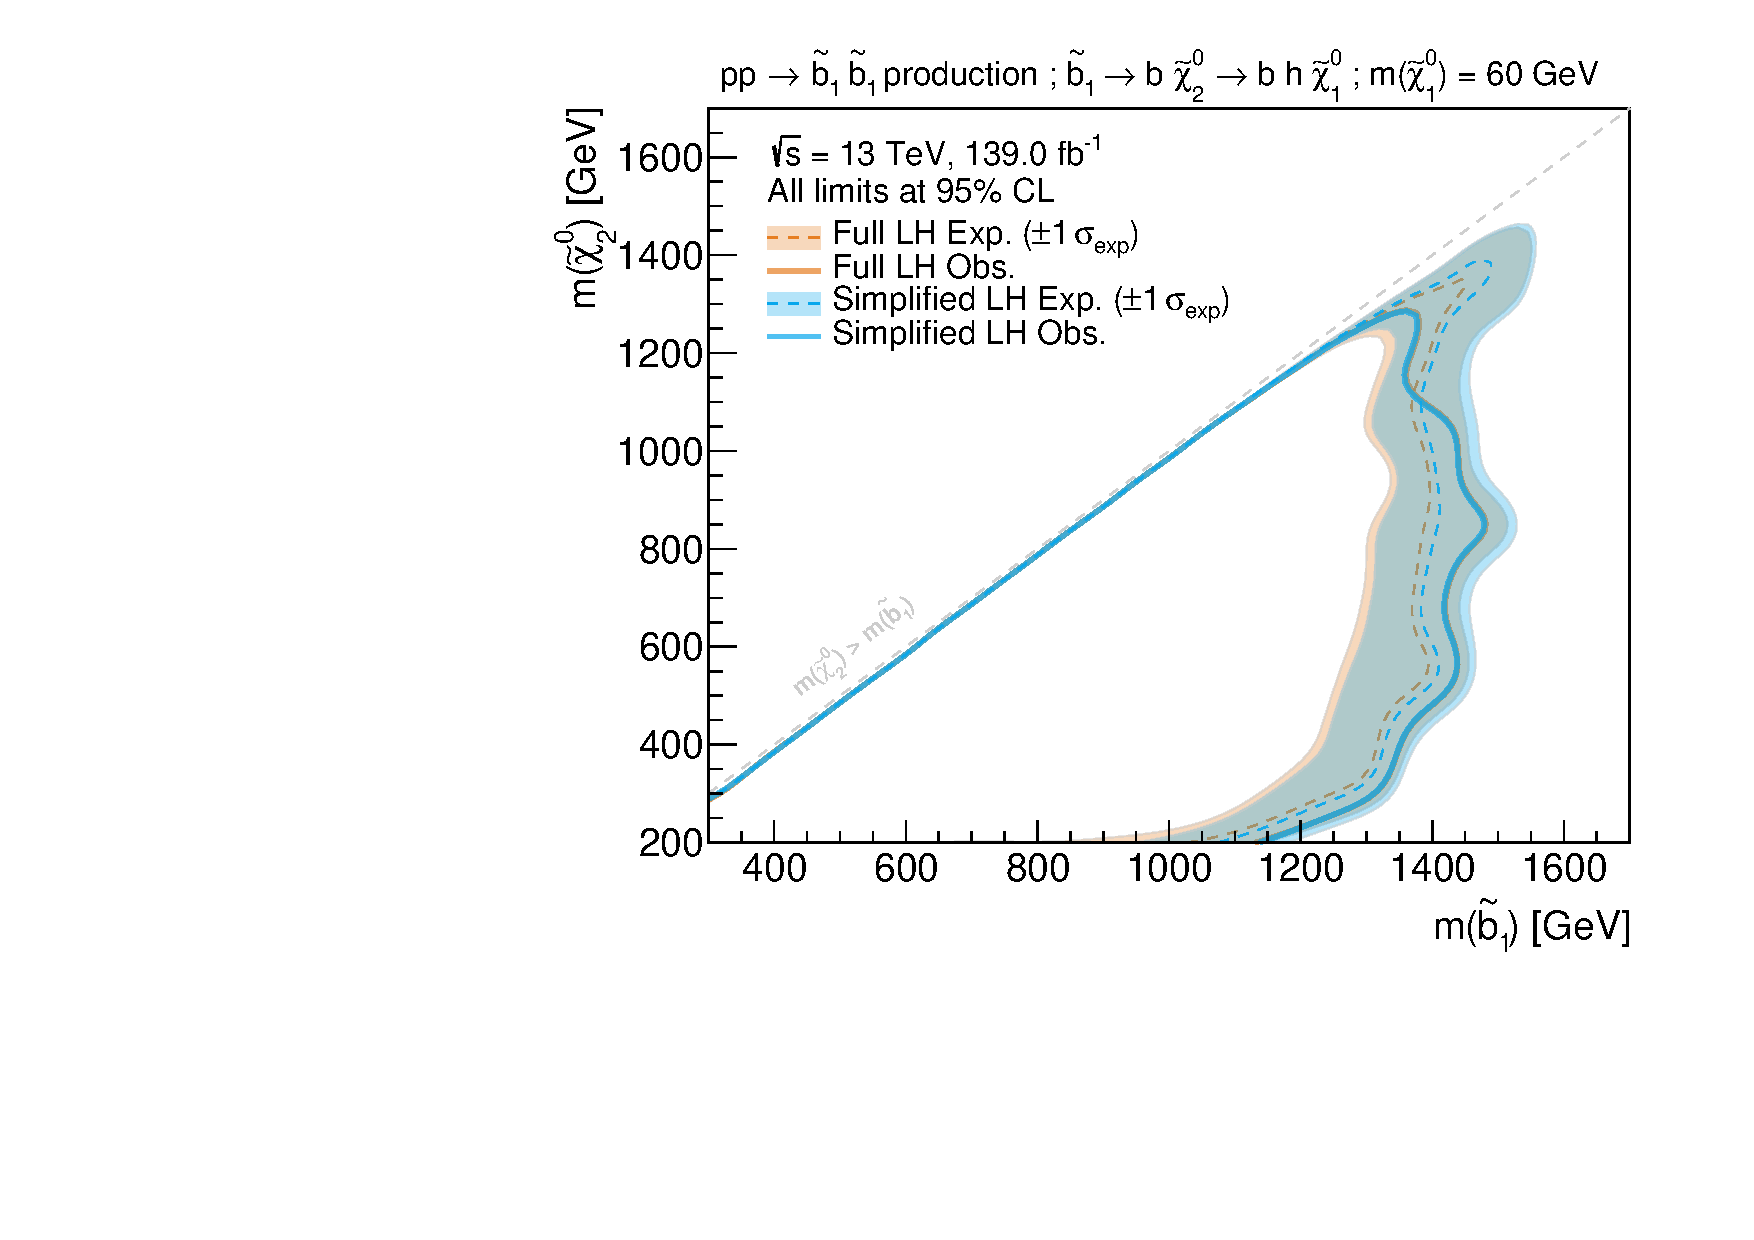
\includegraphics[width=\textwidth]{exclusion_sbottom_noLabel_v2}
		\caption{ATLAS sbottom search~\cite{SUSY-2018-31}\label{fig:results_sbottom}}
	\end{subfigure}\hfill
	\begin{subfigure}[b]{0.5\textwidth}
		\centering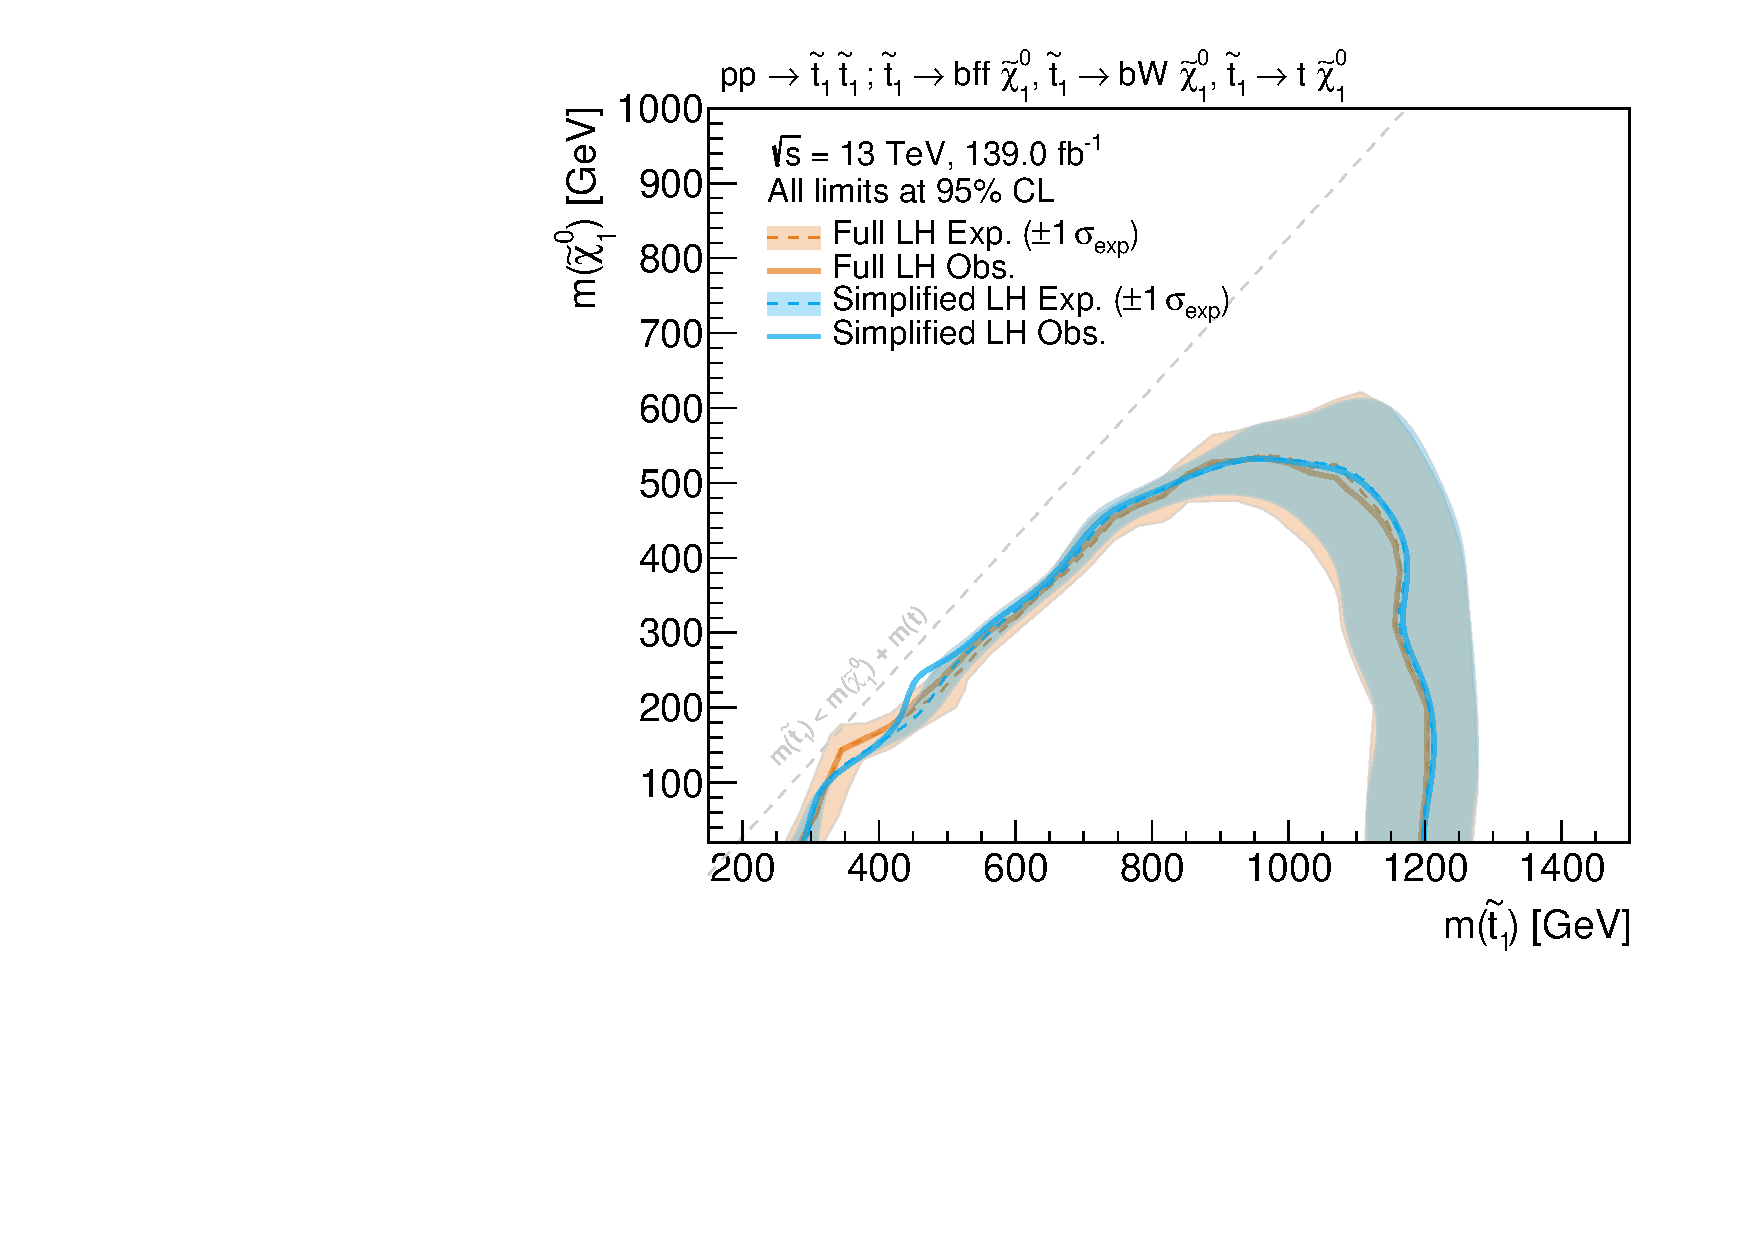
\includegraphics[width=\textwidth]{exclusion_stop1L_noLabel_v2}
		\caption{ATLAS stop search\label{fig:results_stop1L}}
	\end{subfigure}\hfill
	\par\medskip
	\begin{subfigure}[b]{0.5\textwidth}
		\centering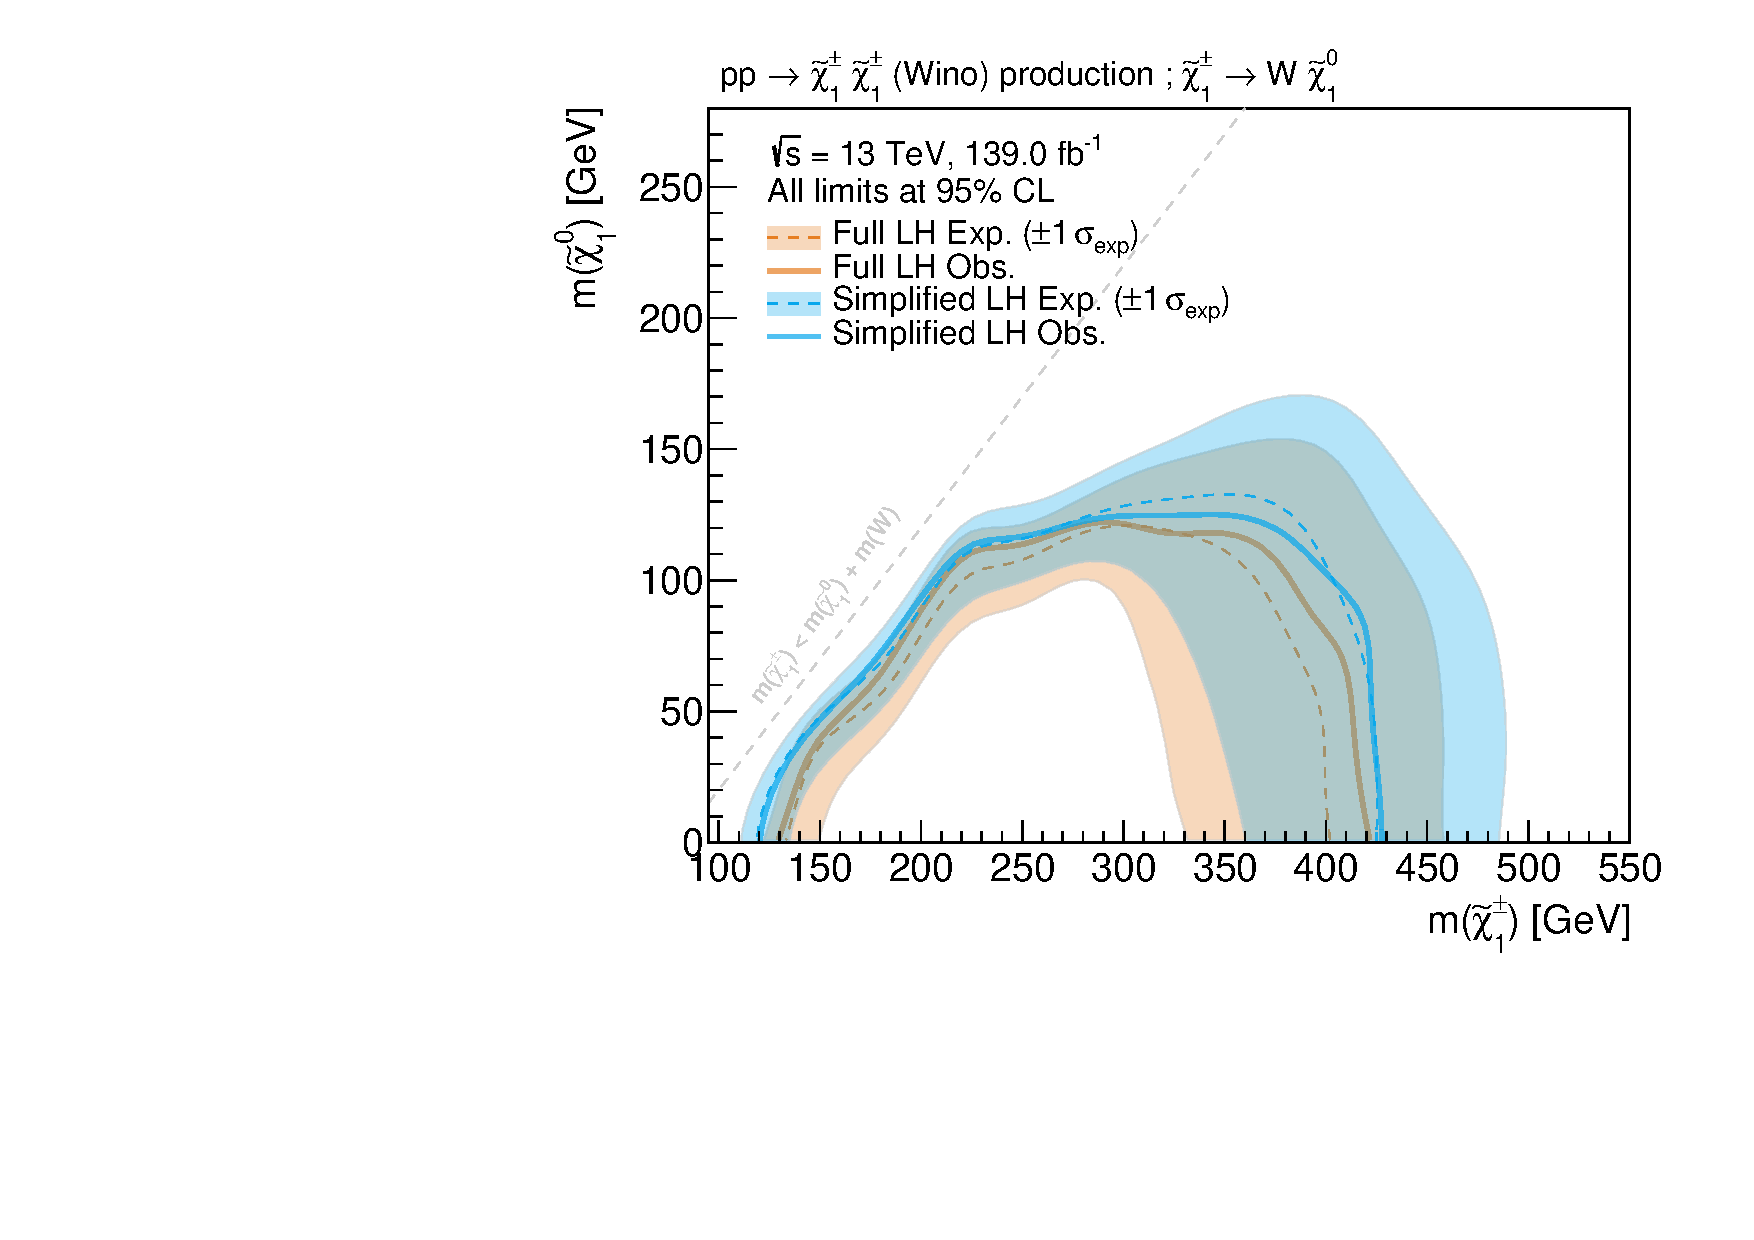
\includegraphics[width=\textwidth]{exclusion_2L0J_noLabel_v2}
		\caption{ATLAS $2\ell$ search~\cite{SUSY-2018-32}\label{fig:results_2L0J}}
	\end{subfigure}\hfill
	\begin{subfigure}[b]{0.5\textwidth}
		\centering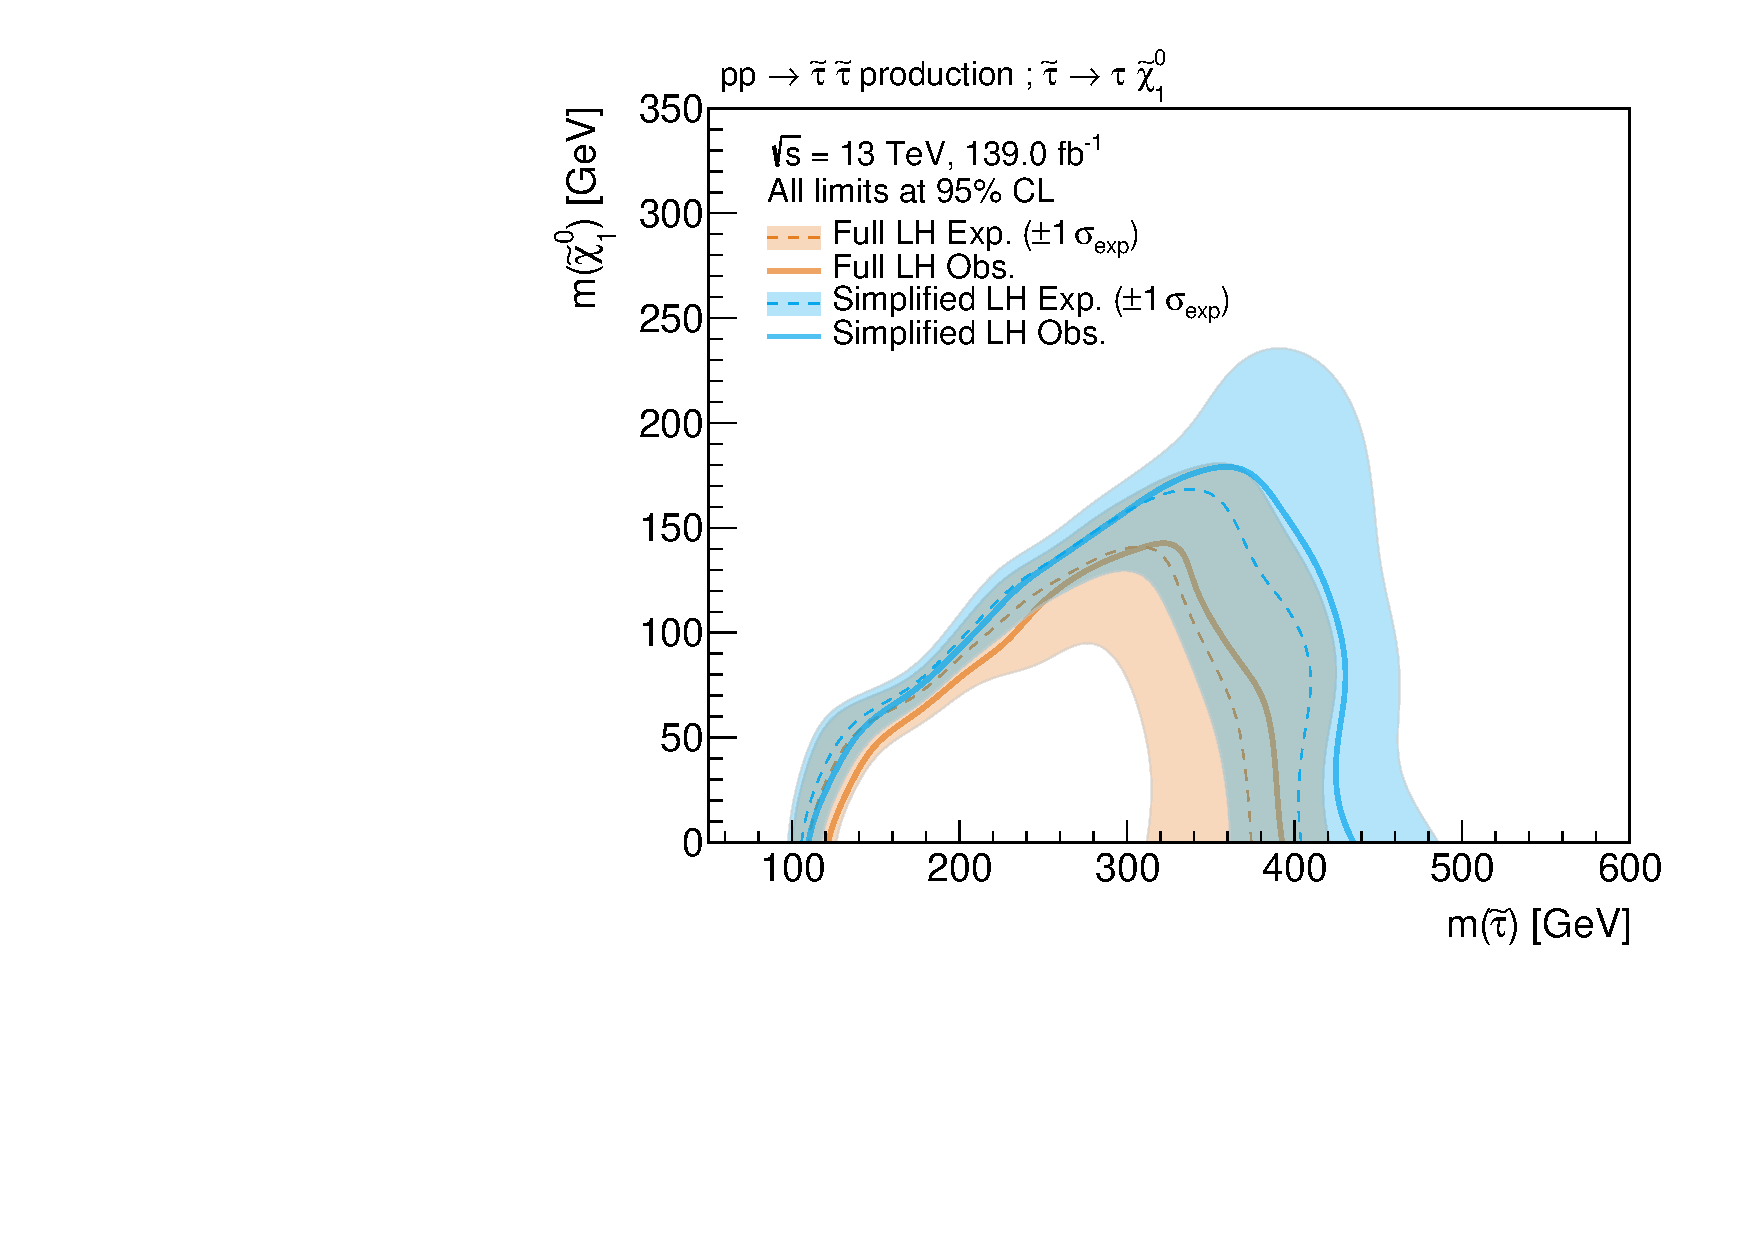
\includegraphics[width=\textwidth]{exclusion_directstaus_noLabel_v2}
		\caption{ATLAS direct stau search~\cite{SUSY-2018-04}\label{fig:results_directstaus}}
	\end{subfigure}\hfill
	\par\medskip
	\begin{subfigure}[b]{0.5\textwidth}
		\centering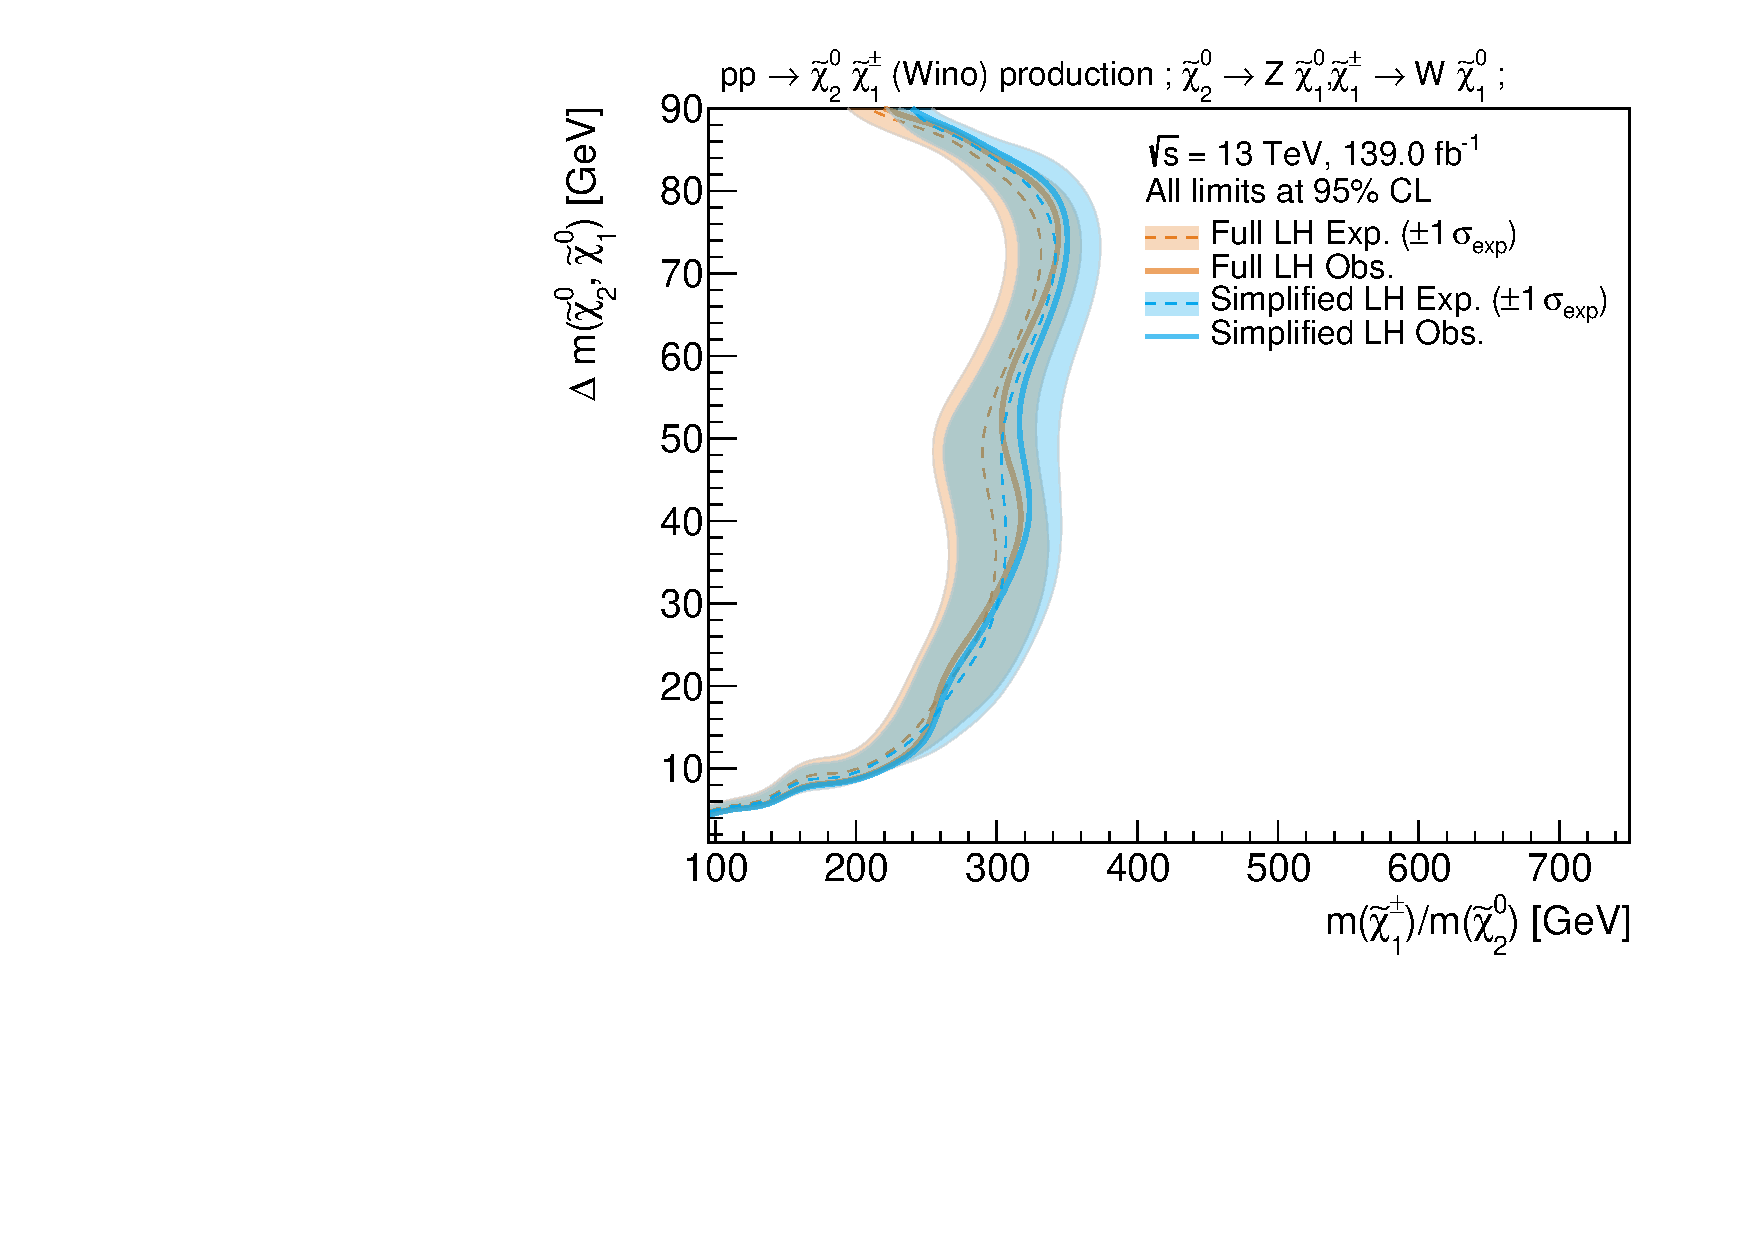
\includegraphics[width=\textwidth]{exclusion_3Loffshell_noLabel_v2}
		\caption{ATLAS $3\ell$ search\label{fig:results_3Loffshell}}
	\end{subfigure}\hfill
	\begin{subfigure}[b]{0.5\textwidth}
		\centering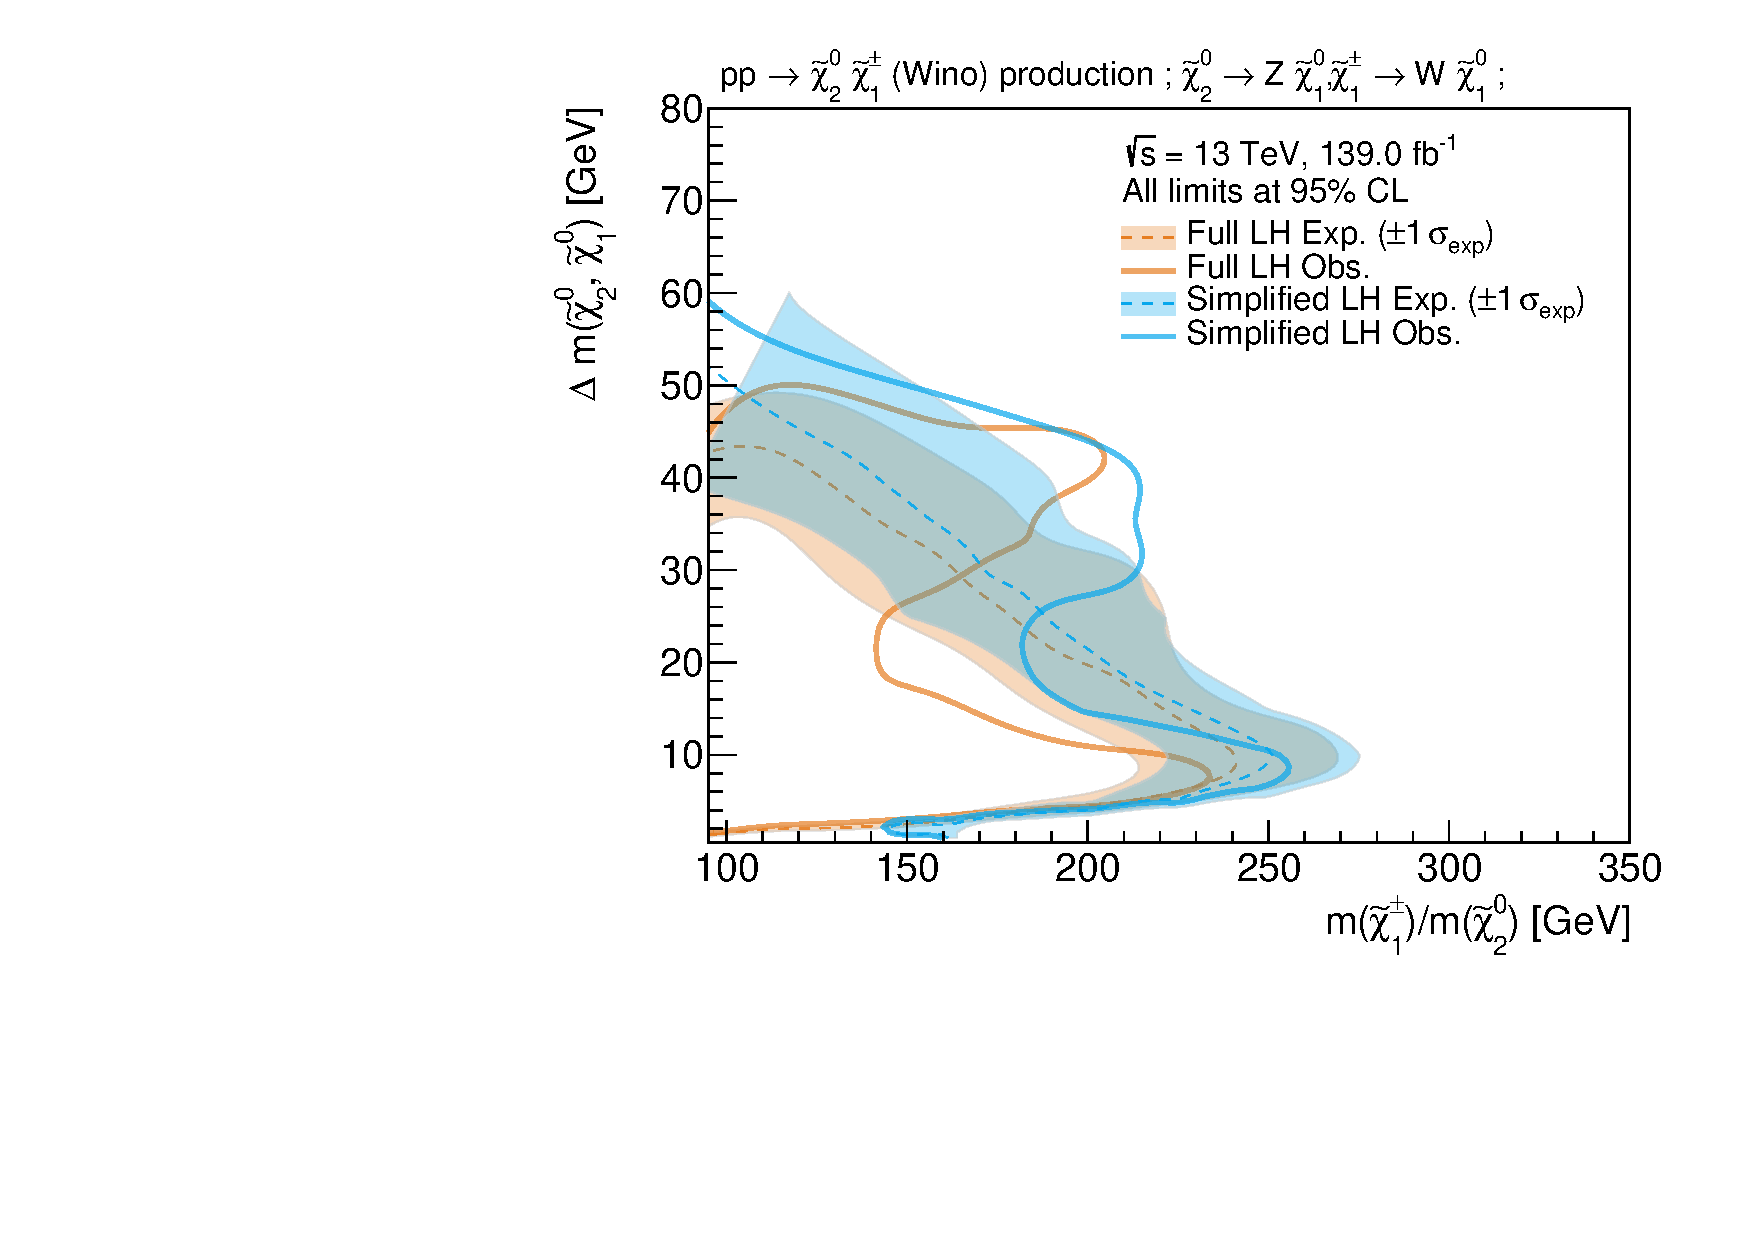
\includegraphics[width=\textwidth]{exclusion_compressed_noLabel_v2}
		\caption{ATLAS compressed search~\cite{SUSY-2018-16}\label{fig:results_compressed}}
	\end{subfigure}\hfill
	\caption{Simplified likelihood results for the different ATLAS searches studied. The results from the simplified likelihood (blue) are compared with the results of the full analysis likelihood (orange). The same reconstruction-level signal inputs are used in both cases. The shorthand notation `\textit{LH}' refers to likelihood.}\label{fig:results_analyses}
\end{figure}

\section{Limitations}\label{sec:simplify_limitations}

Building a well-performing simplified likelihood is not always as straightforward as described in~\cref{sec:building_simplified_likelihoods}, and some analyses require special care when approximated. For example, in the case of the ATLAS compressed search~\cite{SUSY-2018-16}, shown in~\cref{fig:results_compressed}, only a subset of the original analysis signal regions are entering the simplified likelihood, because studies showed this to yield an overall improvement in agreement between the two likelihoods. The straightforward structure of the simplified likelihood is, in this case, not able to reproduce the statistical behaviour of the background model of the full likelihood in the signal regions omitted. As these signal regions were found to only add limited sensitivity to the search, their removal in the simplified likelihood yields an overall improvement in agreement. \Cref{fig:limitations_simplied_compressed} further illustrates the impact of removing these signal regions in the simplified likelihood.

It is worth highlighting again that the simplified likelihood assumes that the total background model can be described by a single sample with a single rate modifier, constrained by a Gaussian and correlated over all bins, with background event rates and uncertainties obtained from a background-only fit using the full likelihood.
This, in particular, assumes that the background model is sufficiently constrained by the large statistics in the \glspl{cr} and that the introduction of signal contributions---especially in the \glspl{sr}---does not significantly change the background model in a way that cannot be replicated with a single background sample where the event rates only depend on a single, constrained nuisance parameter.
Although to some extent tolerable in the full analysis likelihood, such a configuration, where the background model is no longer only mostly constrained by the large statistics in the control regions, is especially problematic for the simplified likelihood.

\improvement{Plot of changing fit behaviour}

An additional limitation arises in cases of significant signal contamination in the \glspl{cr}. In the full likelihood, significant signal contaminations in the \glspl{cr} generally lead to smaller background estimates in the \glspl{sr}, which, in turn, result in conservative exclusion limits given the observed data.
In the simplified likelihood, even with the \glspl{cr} included, the single constrained nuisance parameter does not offer enough degrees of freedom to scale down the background model enough in the $\mu = 1$ hypothesis, resulting in \textit{fake} sensitivity in the \glspl{cr}.
Although it is generally important to limit signal contamination in the \glspl{cr} for the sake of healthy statistical log-likelihood fits, this is especially true in the case of very simplified likelihoods as introduced herein.
In the case of the ATLAS stop search shown in~\cref{fig:results_stop1L}, significant signal contamination of more than 30\% appears for many signal models with $m(\tilde{t}_1) < m(\lsp)+m(t)$, which can thus not be evaluated using the simplified likelihood including control regions\footnote{This is a kinematic region that the analysis is not designed to be sensitive in, hence the \glspl{cr} are not guaranteed to be free of signal contamination.}. In \cref{fig:limitations_simplied_stop1l}, the impact of not applying the simplified likelihood on signal models with significant signal contamination in the region $m(\tilde{t}_1) < m(\lsp)+m(t)$ is shown. In practice, this means that models need to be carefully checked for potential signal contamination in the control regions, and cannot be evaluated using the simplified likelihood in case the signal contamination is found to be too high\footnote{The exact amount of tolerable signal contamination should be explicitly checked on a per-analysis basis. For models exceeding the tolerated amount, the full likelihood can be used instead of the simplified one.}.

\section{Outlook and future prospects}

The simplified likelihoods introduced in this chapter can offer precise and computationally efficient approximations of ATLAS \gls{susy} searches for which the full likelihood in \texttt{JSON} format is available. A publicly available python tool has been developed for generic conversion of any full likelihood in \texttt{JSON} format into the simplified format introduced herein~\cite{simplify}.

The procedure of approximating the statistical model of a search is orthogonal to the truth-level analysis discussed in \cref{sec:truth_analysis} in the sense that both approximations target a different part of the analysis workflow shown in \cref{fig:pipeline_analysis}.
As such, both approaches can be combined into a \textit{simplified analysis} that runs a smeared truth-level analysis in order to determine an estimate for signal event rates, followed by a simplified statistical inference using the simplified likelihood instead of the full statistical model.
\Cref{fig:exclusion_1Lbb_truthInput_BkgSignal_700_200_noLabel} compares the expected and observed exclusion contours obtained in the full \onelepton search published with those obtained with the simplified version of the search, using smeared truth-level analysis and a simplified likelihood.
The agreement observed between the exclusion contours obtained by both analysis versions is noteworthy, especially given the considerable scope of the two-fold approximation applied in the simplified analysis version.
This very simplified analysis will be used in the following chapter to enable a computationally efficient reinterpretation of the \onelepton search in the \gls{pmssm}.

\begin{figure}
\floatbox[{\capbeside\thisfloatsetup{capbesideposition={right,center},capbesidewidth=0.30\textwidth}}]{figure}[\FBwidth]
{\caption{Expected and observed exclusion contours obtained with the full likelihood and reconstruction-level inputs (orange) and the simplified likelihood and smeared truth-level inputs (purple). All statistical and systematic uncertainties on the background and signal are considered for the reconstruction-level contours determined using the full likelihood.}\label{fig:exclusion_1Lbb_truthInput_BkgSignal_700_200_noLabel}}
{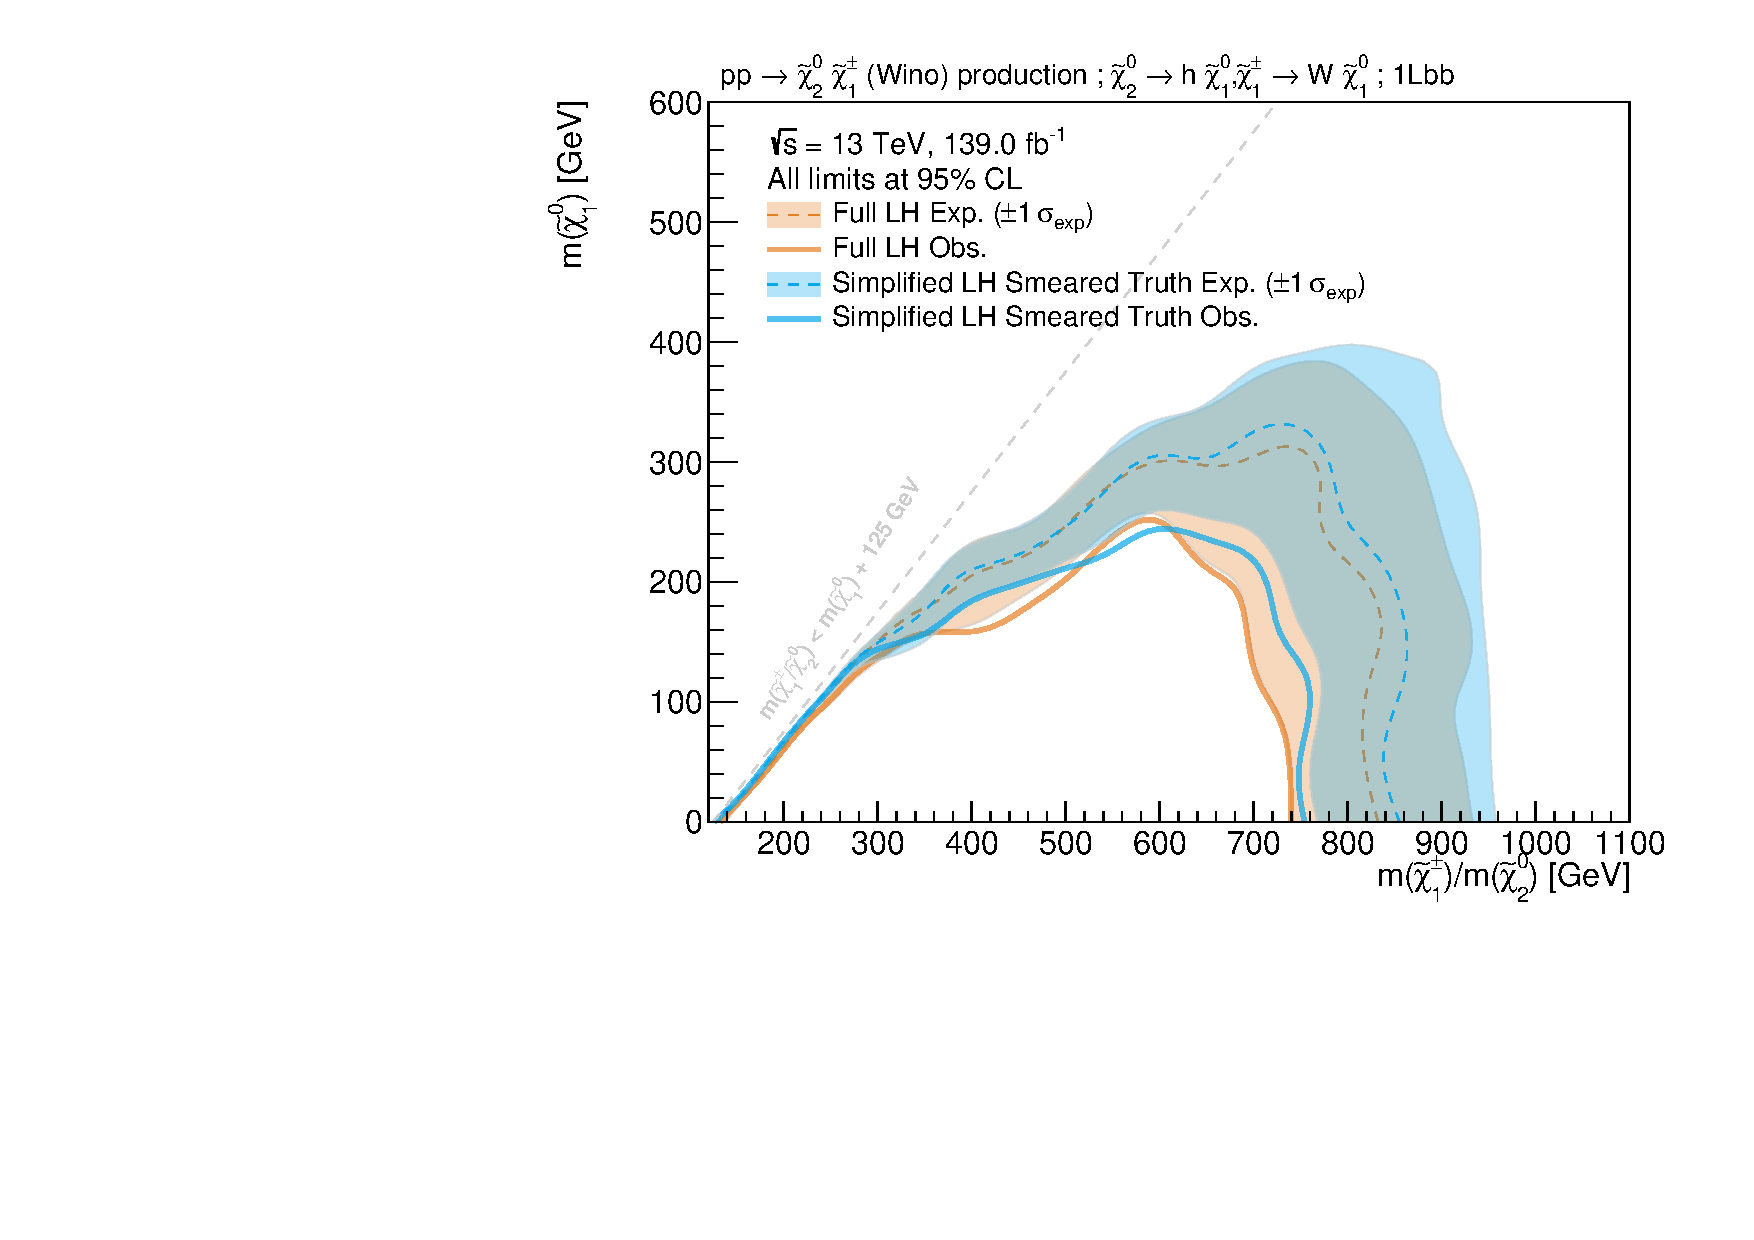
\includegraphics[width=0.65\textwidth]{exclusion_1Lbb_truthInput_BkgSignal_700_200_noLabel}}
\end{figure}


As the full likelihood defines the full statistical model given the observed data in an analysis, other forms of likelihood simplifications can be thought of.
One possible approach worth investigating is the construction of likelihood simplifications using a variable number of nuisance parameters, as opposed to reducing the full set of nuisance parameters to a single one.
In such an approach, a principal components analysis could project the full $N$-dimensional nuisance parameter space onto a number $n\leq N$ principal components maximising the variance of the projected space, \ie resulting in minimal loss in bin-by-bin correlation information.
The $n$ principal components can then be kept separate, while the $N-n$ remaining components can be combined in into a \textit{residual} term\footnote{In a way, the simplified likelihood introduced in this thesis is the special case of this approach where $n=0$ is chosen and none of the principal components are kept separate while all $N$ nuisance parameters are combined into a single term.}.
A similar approach was already introduced in \cref{ch:uncertainties}, where the large number of nuisance parameters related to the \gls{jer} and \gls{jes} uncertainties were reduced to a more manageable set of \textit{effective} nuisance parameters with minimal loss in bin-by-bin correlation information. 

Up until very recently, the only way for physicists outside the collaboration to re-use ATLAS searches for \gls{susy} required building approximations of their statistical models based on lossy projections of the full likelihood.
With ATLAS' recent push to publish full analysis likelihoods, new approaches for approximation of the statistical models are becoming available.
In principle, the full likelihood contains all information necessary for generating a simplified likelihood with a certain degree of compromise between statistical precision and computational efficiency, allowing to find an ideal approximation given constraints on available computing resources of the specific use-case. 

\improvement{ref to simplify}




